% Welcome! This is the unofficial University of Udine beamer template.

% See README.md for more informations about this template.

% This style has been developed following the "Manuale di Stile"
% (Style Manual) of the University of Udine. You can find the
% manual here: https://www.uniud.it/it/ateneo-uniud/ateneo-uniud/identita-visiva/manuali-immagine-stile/manuale-stile

% Note: for some reason, the RGB values specified in the manual
% do NOT render correctly in Beamer, so they have been redefined
% for this document using the high level chromo-optic deep neural 
% quantistic technology offered by Microsoft Paint's color picker.

% We defined four theme colors: UniBrown, UniBlue, UniGold
% and UniOrange. For example, to write some uniud-brownish
% text, just use: \textcolor{UniBrown}{Hello!}

% Note that [usenames,dvipsnames] is MANDATORY due to compatibility
% issues between tikz and xcolor packages.

\documentclass[usenames,dvipsnames,aspectratio=169]{beamer}
\usepackage[utf8]{inputenc}
\usepackage{verbatim}
\usetheme{uniud}

%%% Bibliography
\usepackage[style=authoryear,backend=biber]{biblatex}
\addbibresource{bibliography.bib}

% Author names in publication list are consistent 
% i.e. name1 surname1, name2 surname2
% See https://tex.stackexchange.com/questions/106914/biblatex-does-not-reverse-the-first-and-last-names-of-the-second-author
\DeclareNameAlias{author}{first-last}

%%% Suppress biblatex annoying warning
\usepackage{silence}
\WarningFilter{biblatex}{Patching footnotes failed}
\graphicspath{{graphics/}{graphics/prml/}{implementations/}}

%%% Some useful commands
% pdf-friendly newline in links
\newcommand{\pdfnewline}{\texorpdfstring{\newline}{ }} 
% Fill the vertical space in a slide (to put text at the bottom)
\newcommand{\framefill}{\vskip0pt plus 1filll}


\title[Introduction to Gaussian Processes]{Introduction to \\ Gaussian Processes}
\date[]{\today}
\author[Filipe P. de Farias]{
  Filipe P. de Farias, IC
  \pdfnewline
  \texttt{filipepfarias@fisica.ufc.br}
}
\institute{Teleinformatics Engineering Department, Federal University of Ceará}

\begin{document}
\begin{frame}
\titlepage
\end{frame}

%\begin{frame}{Preamble} 
 The \textbf{Gaussian Processes} are the widely used stochastic processes for modeling dependent data observed over time, space or even tima and space. Here, we'll iniciate our study with a \textbf{Probability and Random Process Theory Review} taking some point to base our journey, going through \textbf{Linear Regression} and finally the \textbf{Gaussian Processes}. \par
 
The material here presented isn't sufficient to guide you over basic probability, so it's recommended to have some knowledge, once we'll just take a simple review.
\end{frame}

\begin{frame}{Outline}
\tableofcontents
\end{frame}

%\include{probability-review}

\section{Linear Regression}\label{sec:linear-regression}
\framecard{\insertsection}
\subsection{Defining models}

\begin{frame}{\insertsubsection}
	\framesubtitle{An initial curve fitting problem}

\begin{itemize}
	\item If we have a set of points in a space that comes from observations of an experiment and we want to predict other points, this could be done with \textbf{\textcolor{UniOrange}{curve fitting}}.
	\item So we could define some strategy to find our model.
\end{itemize}

\begin{block}{Strategy}
	\begin{itemize}
		\item[1] Purpose a \textcolor{UniBlue}{\textbf{model}}, e.g. functions like exponential, polynomial and others.
		\item[2] Train our model with the training data set, finding the \textcolor{UniBlue}{\textbf{unknown parameters}} or \textcolor{UniBlue}{\textbf{weights}}.
	\end{itemize}
\end{block}
\end{frame}


\begin{frame}{\insertsubsection}
	\framesubtitle{An initial curve fitting problem}
	\begin{itemize}
		\item Let's fit the points below by \textcolor{UniOrange}{\textbf{polynomial curve fitting}}.
	\end{itemize}

	\begin{figure}
	\label{fig:plot-fitting-example}
		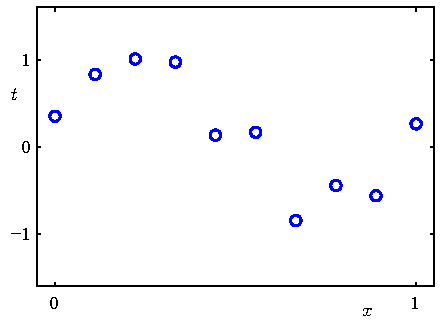
\includegraphics[totalheight=0.75\textheight]{Figure1c2.pdf}
	\end{figure}
\end{frame}

\begin{frame}{\insertsubsection}
	\framesubtitle{Chosing a model}
	\begin{itemize}
		\item Be the model chosen a \textcolor{UniOrange}{\textbf{polynomial}}, we'll have
		\begin{align*}
			y(x,\mathbf{w}) &= w_0x^0 + w_1x^1 + w_2x^2  + ... + w_{M-1}x^{M-1}  = \sum^{M-1}_{j=1} w_j x^j
		\end{align*}	
		\item In general, we could write this \textcolor{UniOrange}{\textbf{weighted sum}} with any other function. In other words, we can put this in terms of $\phi_n(x)=x^n$, where $\phi$ could be other \textcolor{UniOrange}{\textbf{basis function}}.
		\item e.g. we could have different $y$s for different basis functions.
		\begin{align*}
			y(x,\mathbf{w}) &= w_0 \phi_0(x) +w_1 \phi_1(x) +w_2 \phi_2(x)  + ... + w_{M-1} \phi_{M-1}(x) \\
							&= w_0 \exp\left\{ - \frac{(x-\mu_0)^2}{2\sigma^2}\right\} + w_1  \exp\left\{ - \frac{(x-\mu_1)^2}{2\sigma^2}\right\} + \\ & ... + w_{M-1} \exp\left\{ - \frac{(x-\mu_{M-1})^2}{2\sigma^2}\right\} \\
							&= w_0 \sin(0 \cdot x) + w_1 \cos(1 \cdot x) + \\ &... + w_{M_2} \sin((M-2) \cdot x) + w_{M-1} \cos((M-1) \cdot x)
		\end{align*}

\end{itemize}
\end{frame}

\begin{frame}{\insertsubsection}
	\framesubtitle{A non-linear model linear in parameters}
	\begin{itemize}
		\item For simplicity, we'll carry this notation along.
		\begin{align*}
			y(x,\mathbf{w}) &= w_0 \phi_0(x) +w_1 \phi_1(x) +w_2 \phi_2(x)  + ... + w_{M-1} \phi_{M-1}(x) \\
							&= \sum^{M-1}_{j=1} w_j \phi_j(x)
		\end{align*}
		\item We'll evaluate $\phi$ for all $x$, and then project it in the $w$ vector space, then our model could be formed by \textcolor{UniOrange}{\textbf{non-linear}} functions. But, remaining \textcolor{UniOrange}{\textbf{linear on parameters}}.
	\end{itemize}
\end{frame}


\begin{frame}{\insertsubsection}
	\framesubtitle{The model parameters}
\begin{columns}
\begin{column}{0.45\textwidth}
	\begin{itemize}
		\item The chosen model will give us some curve that is needed to adjust such that we'll \textcolor{UniOrange}{\textbf{minimize its distance}} to the \textcolor{UniOrange}{\textbf{targets}} ($t$).
		\item Here, let's define the sum of these distances as \textcolor{UniOrange}{\textbf{cost function}}, or error function, and write it as
		\begin{align*}
			E(\mathbf{w}) \triangleq \frac{1}{2} \sum_{n=1}^N \left\{ y_n -  t_n \right\}^2
		\end{align*}
	\end{itemize}
\end{column}
\begin{column}{0.45\textwidth}  
    \begin{center}
	\centering
	\includegraphics[totalheight=0.4\textheight]{Figure1c3.pdf}
     \end{center}
\end{column}
\end{columns}

\end{frame}
%%%%%%%%%%%%%%%%%%%%%%%%%%%%%%%%%%%
%\begin{frame}{\insertsubsection}

%\textcolor{red}{Insert some \textit{Minkowski} loss.}

%\end{frame}
%%%%%%%%%%%%%%%%%%%%%%%%%%%%%%%%
\begin{frame}{\insertsubsection}
	\framesubtitle{The model parameters}
	\textcolor{UniGold}{\textbf{Why choose a quadratic norm distance?}}
	\begin{figure}
    \begin{subfigure}[t]{0.5\textwidth}
        \centering
        \includegraphics[totalheight=0.35\textheight]{"Figure1.29a".eps}
    \end{subfigure}%
    \begin{subfigure}[t]{0.5\textwidth}
        \centering
        \includegraphics[totalheight=0.35\textheight]{"Figure1.29b".eps}
		\end{subfigure}
		\\
	\begin{subfigure}[t]{0.5\textwidth}
		\centering
		\includegraphics[totalheight=0.35\textheight]{"Figure1.29c".eps}
	\end{subfigure}%
	\begin{subfigure}[t]{0.5\textwidth}
		\centering
		\includegraphics[totalheight=0.35\textheight]{"Figure1.29d".eps}
	\end{subfigure}
	\end{figure}
\end{frame}

\begin{frame}{\insertsubsection}
	\framesubtitle{The model parameters}
	\textcolor{UniGold}{\textbf{Why choose a quadratic norm distance?}}
	\begin{itemize}
		\item The first row figures could me used for the derivations, taking care with some \textcolor{UniOrange}{\textbf{non-continuous derivatives}}.
		\item We'll use the \textcolor{UniOrange}{\textbf{quadratic norm}} because its the minor integer $q$ differentiable, and then the error measures $E$ between the model $y(x,\mathbf{w})$ and the targets $t$ will be euclidean.
		\item More, increasing the value of $q$, the smallests than 1 and bigger than 0 errors between the model and the targets that become irrelevant for $E$.
	\end{itemize}
\end{frame}

\begin{frame}{\insertsubsection}
	\framesubtitle{Matrix form}
	\begin{itemize}
		\item Remembering that
			\begin{align*}
				y(x,\mathbf{w}) &= w_0 \phi_0(x) +w_1 \phi_1(x) +w_2 \phi_2(x)  + ... + w_{M-1} \phi_{M-1}(x) 
			\end{align*}
		\item We'll evaluate for all $x_i$ values, and then put $y_n(x_i,\mathbf{w})$ in the matrix form and get
		\begin{equation*}
			y_n=
			\begin{bmatrix}
				\phi_0(x_n) & \phi_1(x_n) & ... & \phi_{M-1}(x_n)
			\end{bmatrix}
			\begin{bmatrix}
				w_0 & w_1 &  \cdots & w_{M-1}
			\end{bmatrix}^{\top}
		\end{equation*}
		\item And then
		\begin{equation*}
			\underbrace{
				\begin{bmatrix}
				y_1 \\ y_2 \\  \vdots \\ y_N
				\end{bmatrix}
			}_\mathbf{y} = 
			\underbrace{
				\begin{bmatrix}
				\phi_0(x_0) & \phi_1(x_0) & ... & \phi_{M-1}(x_0)   \\ 
				\phi_0(x_1) & \phi_1(x_1) & ... & \phi_{M-1}(x_1)    \\ 
				\vdots & \vdots & \ddots & \vdots \\
				\phi_0(x_{N-1}) & \phi_1(x_{N-1}) & ... & \phi_{M-1}(x_{N-1})  
				\end{bmatrix}
			}_\Phi
			\underbrace{
				\begin{bmatrix}
				w_1 \\ w_2 \\  \vdots \\ w_N
				\end{bmatrix}
			}_\mathbf{w}
		\end{equation*}
		\item This represents the system $\mathbf{y} = \Phi \mathbf{w}$.
\end{itemize}
\end{frame}

\begin{frame}{\insertsubsection}
	\framesubtitle{The cost function}
If
\begin{align*}
E(\mathbf{w}) =& \frac{1}{2} \left( \mathbf{y} - \mathbf{t} \right)^T\left( \mathbf{y} - \mathbf{t} \right)
\end{align*}
where $\mathbf{t} =
\begin{bmatrix}
t_1 & t_2 & ... & t_n
\end{bmatrix}^T
$
%
Then we'll have 
%
\begin{align*}
E(\mathbf{w}) =& \frac{1}{2} \left( \mathbf{y}^T\mathbf{y} -  \mathbf{t}^T\mathbf{y} - \mathbf{y}^T\mathbf{t} + \mathbf{t}^T\mathbf{t} \right) \\
		   =& \frac{1}{2} \left( ( \Phi \mathbf{w})^T( \Phi \mathbf{w}) -  \mathbf{t}^T( \Phi \mathbf{w}) - ( \Phi \mathbf{w})^T\mathbf{t} + \mathbf{t}^T\mathbf{t} \right) \\
		   =& \frac{1}{2} \left( \mathbf{w}^T \Phi^T \Phi \mathbf{w} -  2\mathbf{t}^T \Phi \mathbf{w} + \mathbf{t}^T\mathbf{t} \right)
\end{align*}
this by the fact that $\alpha =  \mathbf{t}^T( \Phi \mathbf{w}) = ( \Phi \mathbf{w})^T\mathbf{t}$, being $\alpha$ a scalar.

\end{frame}

\begin{frame}{\insertsubsection}
In sequence, we'll try to minimize it in terms of the weights ($\mathbf{w}$) by

\begin{align*}
	0 =& \frac{\partial E(\mathbf{w})}{\partial \mathbf{w}} \\
	0 =& \frac{1}{2} \left( 2 \mathbf{w}^T \Phi^T \Phi  -  2\mathbf{t}^T \Phi + 0 \right) \\
	\mathbf{w}^T =&  \mathbf{t}^T \Phi \left( \Phi^T \Phi \right)^{-1} \\
	\mathbf{w} =& \left( \Phi^T \Phi \right)^{-1}\Phi^T \mathbf{t} \\
\end{align*}

Here, we've obtained $\mathbf{w}$ for the curve fitting.

\end{frame}

\begin{frame}
% \vspace{1em}
\lstinputlisting[linerange={3-7,11-12,14-15,17-17,23-23}]{codes/lnReg.m}
\end{frame}

\begin{frame}{\insertsubsection}

\begin{columns}
\begin{column}{0.45\textwidth}
	\visible<1->{A visible effect of the \textit{increase of the complexity} of the model, represented here by $M$, is the \textit{increase of the weights}. We call it \textbf{over-fitting}.}
	
	\vspace{1em}
	\visible<2->{This phenomenon illustrate a method of ever search for the \textit{best estimation for the parameters}.}
	
	\vspace{1em}
	\visible<3->{It's reasonable to see that our model start's to differ from the $y$ and starts to interpolate the noise.}

	
\end{column}
\begin{column}{0.475\textwidth}  %%<--- here
    \begin{center}
	\centering
	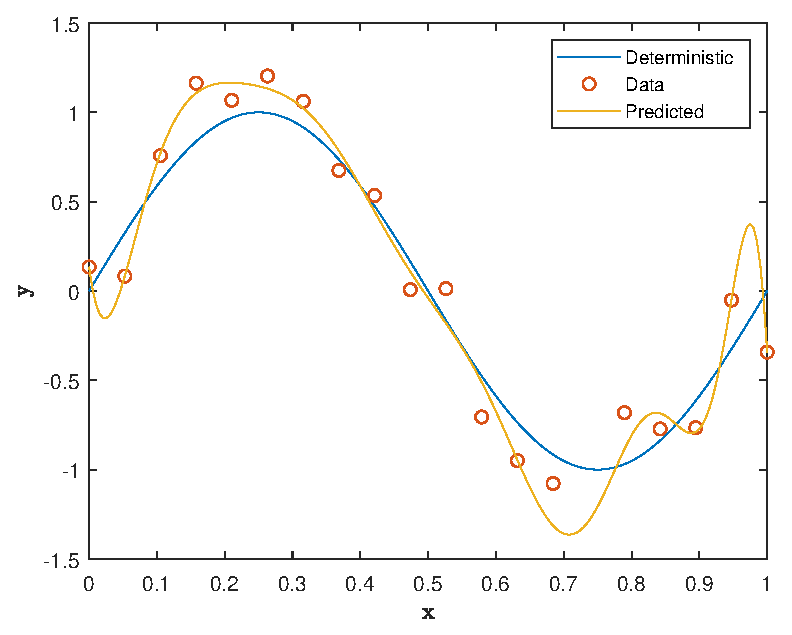
\includegraphics[width=1\linewidth]{lnReg.eps}
     \end{center}
\end{column}
\end{columns}

\end{frame}

\begin{frame}{\insertsubsection}
	
		\begin{figure}
		\label{fig:Erms}
			\includegraphics[totalheight=0.75\textheight]{"Figure1.5".eps}
		\end{figure}
	
	
	\end{frame}

\begin{frame}{\insertsubsection}

\visible<1->{ To control the over-fitting, we try to \textit{regularize} the weights by adding a penalty term ($\lambda$) to error function, by this we force the coefficients to not reach high values.}

\visible<2->{
		\begin{align*}
			\tilde{E}(\mathbf{w}) =&\frac{1}{2} (\mathbf{y}-\mathbf{t})^T(\mathbf{y}-\mathbf{t}) +\frac{\lambda}{2} \mathbf{w}^T\mathbf{w} \\
		   				    =& \frac{1}{2} \left( \mathbf{w}^T \Phi^T \Phi \mathbf{w} -  2\mathbf{t}^T \Phi \mathbf{w} + \mathbf{t}^T\mathbf{t} + \lambda \mathbf{w}^T\mathbf{I}\mathbf{w} \right) \\
	\Rightarrow \frac{\partial E(\mathbf{w})}{\partial \mathbf{w}} =& \frac{1}{2} \left( 2 \mathbf{w}^T \Phi^T \Phi  -  2\mathbf{t}^T \Phi + 0 + 2 \lambda \mathbf{w}^T \mathbf{I} \right) \\
			0 =&  \mathbf{w}^T \Phi^T \Phi  -  \mathbf{t}^T \Phi + \lambda \mathbf{w}^T \mathbf{I} \\
             \mathbf{w} = & \left( \Phi^T \Phi + \lambda \mathbf{I} \right)^{-1} \Phi^T \mathbf{t}
\end{align*}
}

\end{frame}


\begin{frame}
	% \vspace{1em}
	\lstinputlisting[linerange={3-7,12-16,18-18,24-24}]{codes/lnRegRegulated.m}
\end{frame}

\begin{frame}{\insertsubsection}
	
	\begin{figure}
	\label{fig:Erms}
		\includegraphics[totalheight=0.75\textheight]{"Figure1.8".eps}
	\end{figure}


\end{frame}
%%%%%%%%%%%%%%%%%%%%%%%%%%%%%%%%%%%%%%%%%%%%%%%%%
%
\subsection{A probabilistic perspective}
% \begin{frame}{\insertsubsection}
% 	\begin{tikzpicture}[thick]

% 		% Define nodes
% 		\node[latent]                               (t) 
% 			[label=north east:$t_n$] {};
% 		\node[latent, right=of t,draw=red!80, thick] (w) 
% 			[label=north east:$\mathbf{w}$]{};
	
% 		% Connect the nodes
% 		\edge [draw=red!80] {w} {t} ; %
	
% 		% Plates
% 		\plate [draw=blue!80, inner sep=10pt] {} {(t)} {$N$} ;
	
% 	\end{tikzpicture}	
% \end{frame}

\begin{frame}{\insertsubsection}
\begin{columns}
\begin{column}{0.45\textwidth}
	\visible<1->{So, we'll start to look the regression with a probabilistic approach. To encourage you, let's take the sentence.}
	\visible<2->{\vspace{1.5em}
		\begin{block}{Sentence}
		\textit{Having an \textbf{\textcolor{red}{uncertainty}} in the measured value, we could represent it with a  \textbf{\textcolor{red}{probability distribuition}}}.
		\end{block}
   		     }
\end{column}
\begin{column}{0.475\textwidth}  %%<--- here
    \begin{center}
		\visible<3->{
		\includegraphics[totalheight=0.5\textheight]{Figure1c16.pdf}
		}
     \end{center}
\end{column}
\end{columns}
\end{frame}

\begin{frame}{\insertsubsection}
\begin{columns}
\begin{column}{0.45\textwidth}
	\visible<1->{Let's go back to the initial problem of curve fitting. Each observation of the phenomenon is described with a random variable whose \textit{mean} is given by $y(x,\mathbf{w})$, and the \textit{variance} by $\beta$. }
	\visible<2->{\vspace{1.5em}\\
			Then, we want to obtain the probability of the \textit{targets}, given some parameters, in this case $\mathbf{x}$, $\mathbf{w}$ and $\beta$.}
\end{column}
\begin{column}{0.475\textwidth}  %%<--- here
    \begin{center}
		\visible<1->{
		\includegraphics[totalheight=0.5\textheight]{Figure1c16.pdf}
		}
     \end{center}
\end{column}
\end{columns}
\end{frame}

\begin{frame}{\insertsubsection}	
	\visible<1->{So, if we consider that our conditions are such that being the random variables independent and identically distributed, we can say that our \textit{joint probability} is given by
	\begin{equation*}
		p(t | x, \mathbf{w}, \beta) \Rightarrow p(\mathbf{t} | \mathbf{x}, \mathbf{w}, \beta) = \prod_{n=1}^N p \left( t_n | x_n, \mathbf{w}, \beta \right)
	\end{equation*}
	}
	\visible<2->{Let's assume we have a distribution such that $p( \mathbf{t}| \mathbf{x}, \mathbf{w}, \beta)$. Our goal is, given the \textit{parameters}, maximize the \textit{probability} of the \textit{targets} given the \textit{parameters}. An approach to do this use the fact that
	}
	\visible<2->{
	\begin{equation*}
	\int_\infty ^{-\infty} p(x) dx = 1 \text{ and } p(x) \geq 0
	\end{equation*}}
\end{frame}

\begin{frame}{\insertsubsection}

	Seen this, we're supposing that $p$ could assume values much smaller than one. To avoid computational singularity and for future purposes, we'll take the logarithmic probability. And then
	\begin{equation*}
		\ln \left( p( \mathbf{t}| \mathbf{x}, \mathbf{w}, \beta) \right)
	\end{equation*}
	Reminding that
	\begin{equation*}
		p(\mathbf{t} | \mathbf{x}, \mathbf{w}, \beta) = \prod_{n=1}^N p \left( t_n | x_n, \mathbf{w}, \beta \right)
	\end{equation*}
	Implies that
	\begin{equation*}
		\ln \left( p( \mathbf{t}| \mathbf{x}, \mathbf{w}, \beta) \right) = \sum_{n=1}^N \ln \left(   p \left( t_n | x_n, \mathbf{w}, \beta \right) \right)
	\end{equation*}
\end{frame}

\begin{frame}{\insertsubsection}

\begin{columns}
\begin{column}{0.45\textwidth}
	\visible<1->{To proceed, we need to know what distribution $p$ is. Let's choose the \textbf{\textcolor{UniGold}{Gaussian distribution}}. \\ }
\end{column}
\begin{column}{0.475\textwidth}  %%<--- here
    \begin{center}
		\visible<1->{
		\includegraphics[totalheight=0.5\textheight]{Figure1c16.pdf}
		}
     \end{center}
\end{column}
\end{columns}
\end{frame}

\begin{frame}{\insertsubsection}
\begin{columns}
\begin{column}{0.45\textwidth}

	\visible<1->{The \textbf{\textcolor{UniGold}{Gaussian distribution}} comes from many different contexts, as the one that maximize the entropy among of all ones with fixed variance and from the sum of multiple random variables with finite variance. \\ }
	
\end{column}
\begin{column}{0.475\textwidth}  %%<--- here
    \begin{center}
		\visible<1->{
		\includegraphics[width=1\linewidth]{"Figure1.13".pdf}
		}
     \end{center}
\end{column}
\end{columns}
\end{frame}

\begin{frame}{\insertsubsection}

\begin{block}{One-dimensional Gaussian distribution}
\begin{equation*}
	\mathcal{N}(x | \mu, \sigma^2) = \frac{1}{(2 \pi \sigma^2)^{1/2}} \exp \left\{ -\frac{1}{2 \sigma^2} (x- \mu)^2 \right\} > 0
\end{equation*}
where $\mu$ is the mean and $\sigma^2$ the variance.
\end{block}

\end{frame}

\begin{frame}{\insertsubsection}

Now, back to the discussion of the maximization of 
\begin{equation*}
		\ln \left( p( \mathbf{t}| \mathbf{x}, \mathbf{w}, \beta) \right) = \sum_{n=1}^N \ln \left(   p \left( t_n | x_n, \mathbf{w}, \beta \right) \right)
\end{equation*}

\visible<2->{Reminding that
\begin{equation*}
\mathcal{N}(x | \mu, \sigma^2) = \frac{1}{(2 \pi \sigma^2)^{1/2}} \exp \left\{ -\frac{1}{2 \sigma^2} (x- \mu)^2 \right\}
\end{equation*}
we can state a Gaussian distribution for each target and then
}
\visible<3->{
\begin{equation*}
 p( t| \mathbf{x}, \mathbf{w}, \beta) = \mathcal{N} \left( t | y(\mathbf{x}, \mathbf{w}), \beta^{-1} \right)
\end{equation*}
}

\end{frame}

\begin{frame}{\insertsubsection}
\visible<1->{
And then, from the \textit{joint probability} of the Gaussians distributions

\begin{equation*}
		\ln \left( p( \mathbf{t}| \mathbf{x}, \mathbf{w}, \beta) \right) = \sum_{n=1}^N - \frac{1}{2} \ln (2 \pi) + \sum_{n=1}^N \frac{1}{2} \ln \beta - \sum_{n=1}^N \frac{\beta}{2} (x_n -  y(x_n, \mathbf{w}))^2
\end{equation*}

From this, we could obtain the \textbf{maximum likelihood}, or the \textit{best estimation for the parameters}, taking the derivatives of the log probability to zero, according to the terms $\beta$ and $\mathbf{w}$, our model parameters.
}
%Maximizing with respect to $\beta$, we'll have 

%\begin{equation*}
%		\frac{1}{\beta_{ML}} = \frac{1}{N} \sum^N_{n=1} \left\{ y(x_n, \mathbf{w}_{ML}) - t_n \right\}^2
%\end{equation*}
%
%where $\beta_{ML}$ is the precision parameter for the maximum likelihood for the conditional Gaussian distribution.
\end{frame}

\begin{frame}{\insertsubsection}
We could observe that taking the derivative with respect to $\mathbf{w}$, our expression becomes closer to the \textit{error function} presented previously, added the dependency of $\beta$
\begin{align*}
	E(\mathbf{w}) \triangleq \frac{1}{2} \sum_{n=1}^N \left\{ y_n -  t_n \right\}^2
\end{align*}
Then some behaviors could be expected, as the \textbf{over-fitting}.
%Maximizing with respect to $\beta$, we'll have 
%\begin{equation*}
%		\frac{1}{\beta_{ML}} = \frac{1}{N} \sum^N_{n=1} \left\{ y(x_n, \mathbf{w}_{ML}) - t_n \right\}^2
%\end{equation*}
%
%where $\beta_{ML}$ is the precision parameter for the maximum likelihood for the conditional Gaussian distribution.
\end{frame}

\begin{frame}{\insertsubsection}
	We'll obtain the best $\beta$ by
	\begin{equation*}
	\frac{1}{\beta_{ML}} = \frac{1}{N} \sum^N_{n=1} \left\{ y(x_n, \mathbf{w}_{ML}) - t_n \right\}^2
	\end{equation*}
	remembering that $\mathbf{w}_{ML}$ is already known from the regular linear regression.	
\end{frame}

\begin{frame}{\insertsubsection}

At this point, we have a probabilistic model and we may want to predict values for $x$. Then, we need a \textit{predictive distribution}. \\
\vspace{1em}
Let's say we have the probabilities of some idea we desire to update it in the light of some new evidence. This could be done with \textbf{Bayes' Rule}, to convert a \textit{prior} probability in a \textit{posterior} probability and put some uncertainty in the parameters too. \\
\end{frame}

\begin{frame}{\insertsubsection}
Mathematically, by Bayes' Rule, we could infer
\visible<2->{
\begin{equation*}
\underbrace{p\left( \mathbf{w} | \mathbf{x}, \mathbf{t}, \alpha, \beta \right)}_{\text{posterior}} \propto \underbrace{p\left(  \mathbf{t} |\mathbf{w} ,\mathbf{x}, \beta \right)}_{\text{likelihood}}  \underbrace{p\left( \mathbf{w} | \alpha \right)}_{\text{prior}}
\end{equation*}
}
\visible<3->{
and for simplicity, consider the follow prior for $\mathbf{w}$
\begin{equation*}
p \left( \mathbf{w} | \alpha \right) = \mathcal{N} \left( \mathbf{w} | \boldsymbol{0}, \alpha^{-1} \mathbf{I} \right) = \left(  \frac{\alpha}{2 \pi}\right) ^{(M+1)/2} \exp \left\{ - \frac{\alpha}{2} \mathbf{w}^T \mathbf{w} \right\}
\end{equation*}
where $\alpha$ the precision of the distribution and $M+1$ is the dimension of $\mathbf{w}$, for a polynomial of $M^{th}$ order. Variables such $\alpha$ are called \textit{hyperparameters} and control the distribuition of model parameters.}
\end{frame}

\begin{frame}{\insertsubsection}
By this, we can find a distribution and its maximum, or most probable value of $\mathbf{w}$ given the data taking the minimum of the negative logarithm of the infered expression, that will lead us to a term

\begin{equation*}
\sum^N_{n=1} \left\{ y(x_n, \mathbf{w}) - t_n \right\}^2 + \frac{\alpha}{2} \mathbf{w}^T\mathbf{w} + \text{const.}
\end{equation*}

Note that if we consider $\lambda = \alpha / \beta$, this will back to the regularized form of \textit{least squares}. This technique is called \textit{maximum posterior} (MAP).
\end{frame}

\begin{frame}{\insertsubsection}

So, observe that even making some probabilistic assumptions, we don't have yet a fully bayesian model, given that finding the \textit{maximum likelihood}, we're finding only the parameters given one model such that maximize our targets probabilities. Furthermore, even with some probabilistic assumptions, our model still have a \textbf{over-fitting} problem, given that we obtained the same expressions for the simple regression, adding some constants.\\
\vspace{1em}
The next step is put some \textbf{uncertainty in predictive model}, and makes adjustments in the light of our new evidences. By that we could obtain a "more Bayesian" model, in other words, a \textcolor{UniGold}{\textbf{Bayesian Linear Regression}}.

\end{frame}

%\begin{frame}{\insertsubsection}
%	\visible<1->{Let's take a look at the Bayes Theorem}
%	
%	\visible<2->{
%	\begin{block}{Bayes Theorem}{
%			\begin{equation*}\label{bayes_theorem}
%				\visible<2->{ p(\mathbf{w}|\mathcal{D}) = \frac{p(\mathcal{D}| \mathbf{w}) p(\mathbf{w}) } {  p(\mathcal{D}) } } 
%			\end{equation*}
%			}
%	\end{block}
%	\visible<3->{The new role of Bayes Theorem here is the fact that we could obtain new, or better, probability distribuitions for the weights in light of an determined data set $\mathcal{D}$.}
%	}
%\end{frame}

%\begin{frame}{\insertsubsection}
%	\visible<1->{\textbf{\textcolor{UniGold}{At this time, it's important to point out some things. \\}}}
%	\vspace{1.5em}
%	\visible<2->{When we write $ p \left( t_n | x_n, \mathbf{w}, \beta \right)$, we assume a probability distribuition over the parameters $\mathbf{w}$ and $\beta$ too.\\}
%	\vspace{1.5em}
%	\visible<3->{Then we could observe that we'll obtain a \textbf{discrete distribution of functions} in their \textit{parameters}.\\}
%	\vspace{1.5em}
%	\visible<4->{So, here is where the Bayes Theorem plays an important role by \textbf{adjusting} these \textit{parameters} as we obtain evidences.}
%\end{frame}
%
%\begin{frame}{\insertsubsection}
%	\visible<1->{Taking some steps back, let's re-visit the \textbf{Curve Fitting}. There, the strategy was minimize the error function.\vspace{1.5em} \\}
%	\visible<2->{Now we'll try to view the same problem with a \textit{probabilistic perspective}. We're trying to make predictions for the target value $\mathbf{t}$ given some new values of $x$.\vspace{1.5em} \\}
%
%\end{frame}


%\begin{frame}{\insertsubsection}
%	And taking the derivatives with respect to $\beta$ to minimize the error	
%		\begin{align*}
%		\visible<1->{
%			\frac{\partial}{\partial \beta}\ln \left( p( \mathbf{t}| \mathbf{x}, \mathbf{w}, \beta) \right) &=0 } \\
%		\visible<2->{
%			 -\frac{1}{2} \sum^N_{n=1} \left\{ y(x_n,\mathbf{w} -t_n ) \right\}^2 + \frac{N}{2}\frac{1}{\beta} &= 0 \\  }
%		\visible<3->{
%			 \frac{1}{N} \sum^N_{n=1} \left\{ y(x_n,\mathbf{w} -t_n ) \right\}^2  &= \frac{1}{\beta_{ML}}  }
%		\end{align*}
%	\visible<4->{
%	Where $\beta_{ML}$ is the maximum likelihood.}
%
%\end{frame}

\section{Bayesian Linear Regression}

\framecard{\insertsection}

\subsection{Bayesian statistics}

\begin{frame}{\insertsection}
	\framesubtitle{Bayesian vs. Frequentist statistics}
	
	\textcolor{UniGold}{\textbf{What if we assume not knowing the data exactly?}}

	\begin{columns}
		\begin{column}{0.475\textwidth}
			\begin{itemize}
				\item The principle of the Bayesian statistics is express our \textcolor{UniOrange}{\textbf{degree of belief}} in an event.
				\item This belief could be based on some \textcolor{UniOrange}{\textbf{prior}} knowledge about the event or personal beliefs.
				\item This differs from frequentist statistics, where the probability is based on the number of trials.
				\item Suppose a die to be thrown once
			\end{itemize}
			\only<1>{
			\begin{block}{Frequentist}
				There's empiric evidence that similar dice thrown in past produce similar outcomes with the same frequency.
			\end{block}}
			\only<2>{
			\begin{exampleblock}{Bayesian}
				The last argument is right, but the \textcolor{UniBlue}{\textbf{belief of the observer}} it's important to the statistics.
			\end{exampleblock}}
			\end{column}
			\begin{column}{0.475\textwidth}   
				\centering
				\begin{figure}
					\includegraphics[width=1\linewidth]{"Triplot-of-prior-likelihood-and-posterior"}
				\caption{\cite{AksuAnil2018}}
				\end{figure}
			\end{column}
		\end{columns}
\end{frame}
	
\begin{frame}{\insertsection}
	\framesubtitle{Bayes' Rule}

	\begin{itemize}
		\item The main idea of the Bayesian approach is put some \textcolor{UniOrange}{\textbf{uncertainty}} over the parameters and make \textcolor{UniOrange}{\textbf{inferences}}, i.e. obtain some statistics in light over the data.
		\item This principle is elucidated by the Bayes' Rule
		\begin{equation*}
			\overbrace{p(\mathbf{w}|\mathbf{t})}^{posterior} = \frac{p(\mathbf{t}|\mathbf{w}) p(\mathbf{w})}{p(\mathbf{t})} = \frac{\overbrace{p(\mathbf{t}|\mathbf{w})}^{\text{\textit{likelihood}}} \overbrace{p(\mathbf{w})}^{\text{\textit{prior}}}}{\underbrace{\int p(\mathbf{t}|\mathbf{w}) p(\mathbf{w}) d\mathbf{w}}_{\text{\textit{marginal distribution}}}}
		 \end{equation*}
		 where we assume some uncertainty over the parameters, i.e. a probability density function $p(\mathbf{w})$.
		 \item We'll use the knowledge about the data with the \textcolor{UniOrange}{\textbf{likelihood function}} and some previous knowledge, or \textcolor{UniOrange}{\textbf{prior}}, that we have about the parameters to obtain the knowledge considering these two, or \textcolor{UniOrange}{\textbf{posterior}}.
		 \item This is called \textcolor{UniOrange}{\textbf{Bayesian Inference}}.
	\end{itemize}
% \visible<2->{
% \begin{equation*}
% \underbrace{p\left( \mathbf{w} | \mathbf{x}, \mathbf{t}, \alpha, \beta \right)}_{\text{posterior}} \propto \underbrace{p\left(  \mathbf{t} |\mathbf{w} ,\mathbf{x}, \beta \right)}_{\text{likelihood}}  \underbrace{p\left( \mathbf{w} | \alpha \right)}_{\text{prior}}
% \end{equation*}
% }
% \visible<3->{
% and for simplicity, consider the follow prior for $\mathbf{w}$
% \begin{equation*}
% p \left( \mathbf{w} | \alpha \right) = \mathcal{N} \left( \mathbf{w} | \boldsymbol{0}, \alpha^{-1} \mathbf{I} \right) = \left(  \frac{\alpha}{2 \pi}\right) ^{(M+1)/2} \exp \left\{ - \frac{\alpha}{2} \mathbf{w}^{\top} \mathbf{w} \right\}
% \end{equation*}
% where $\alpha$ the precision of the distribution and $M+1$ is the dimension of $\mathbf{w}$, for a polynomial of $M^{th}$ order. Variables such $\alpha$ are called \textit{hyperparameters} and control the distribuition of model parameters.}
\end{frame}

\begin{frame}{\insertsection}
	\framesubtitle{Maximum \textit{a posteriori}}
	\begin{itemize}
		\item We can introduce the \textcolor{UniOrange}{\textbf{maximum \textit{a posteriori}}} (MAP) as the direct estimator for the Bayes' Rule.
		\item The approach is similar to what was done by maximizing the likelihood function, but now maximizing the posterior distribuition of the parameters given the data.
		\item We consider the \textcolor{UniOrange}{\textbf{marginal distribution}} $p(\mathbf{t})$ being a constant in the parameters
	
		\begin{equation*}
			p\left( \mathbf{w} | \mathbf{x}, \mathbf{t} \right) \propto p\left(  \mathbf{t} |\mathbf{w} ,\mathbf{x} \right)p\left( \mathbf{w} \right)
		\end{equation*}

		\item Here, we'll consider out prior knowledge about the parameters being
		
		\begin{equation*}
			\mathbf{w} \sim \mathcal{N} \left( \mathbf{0}, \alpha^{-1} \mathbf{I} \right)
		\end{equation*}

		\item We obtain by the derivative w.r.t. $\mathbf{w}$ of the negative log that
		
		\begin{equation*}
			\sum_{n=1}^N \frac{\beta}{2} (t_n -  y(x_n, \mathbf{w}))^2 + \frac{\alpha}{2} \mathbf{w}^{\top}\mathbf{w} + \text{const.}
		\end{equation*}

		what is similar to the regularized linear regression considering $\lambda = \alpha/\beta$.
	\end{itemize}
\end{frame}

\begin{frame}{\insertsection}
	\framesubtitle{A fully Bayesian approach}

	\textcolor{UniGold}{\textbf{Aren't we ignoring possible solutions?}}
	\begin{itemize}
		\item The main idea in the Bayesian approach is that our knowledge is in the \textcolor{UniOrange}{\textbf{statistics}} and not in a singular value.
		\item With MAP we just consider the \textcolor{UniOrange}{\textbf{most probable}} value of a full distribution of possible values.
		\item In the next we'll obtain the statistics of the distributions involved in Bayes' Rule, including the posterior.
		\item But before, we need some tools...
	\end{itemize}
\end{frame}


\begin{frame}{\insertsection}
	\framesubtitle{Some Gaussian algebra}

	\begin{block}{Partitioned Gaussians}
		Be $\mathbf{x}$ a n-dimensional vector with a Gaussian distribution $\mathcal{N}\left( \mathbf{x} | \boldsymbol{\mu}, \boldsymbol{\Sigma} \right)$, then the partitioned will be
  
		\begin{equation*}
			\mathbf{x}=
			\begin{pmatrix}
			\mathbf{x}_a \\  
			\mathbf{x}_b 
			\end{pmatrix}
			,\quad 
			\boldsymbol{\mu}=
			\begin{pmatrix}
			\boldsymbol{\mu}_a \\
			\boldsymbol{\mu}_b
			\end{pmatrix}
			,\quad 
			\boldsymbol{\Sigma}=
			\begin{pmatrix}
			\boldsymbol{\Sigma}_{aa} & \boldsymbol{\Sigma}_{ab}  \\
			\boldsymbol{\Sigma}_{ba} & \boldsymbol{\Sigma}_{bb}
			\end{pmatrix}
			.
		\end{equation*}

		Preserved the symmetry $\boldsymbol{\Sigma}^\top = \boldsymbol{\Sigma}$, we say the covariance matrix is positive definite. And be the multivariate Gaussian

		\begin{equation*}
			\mathcal{N}(\mathbf{x} | \boldsymbol{\mu}, \boldsymbol{\Sigma})=\frac{1}{(2 \pi)^{n / 2}} \frac{1}{ \left( \det \boldsymbol{\Sigma} \right) ^{1 / 2}} \exp \left\{-\frac{1}{2}(\mathbf{x}-\boldsymbol{\mu})^{\mathrm{T}} \boldsymbol{\Sigma}^{-1}(\mathbf{x}-\boldsymbol{\mu})\right\}
		\end{equation*}

		We define too, just for convenience of work, the precision matrix $\boldsymbol{\Lambda}$ by

		\begin{equation*}
			\boldsymbol{\Lambda} = 
			\begin{pmatrix}
			\boldsymbol{\Lambda}_{aa} & \boldsymbol{\Lambda}_{ab}  \\
			\boldsymbol{\Lambda}_{ba} & \boldsymbol{\Lambda}_{bb}
			\end{pmatrix} 
			\equiv \boldsymbol{\Sigma}^{-1}
		\end{equation*}

		assuming all matrices have inverses.
	\end{block}
\end{frame}

\subsection{Some Gaussian algebra}

\begin{frame}{\insertsection}
	\framesubtitle{Some Gaussian algebra}

	\begin{block}{Closure under linear transformations and marginalization}
		Being $\mathbf{x}_b$ conditioned on $\mathbf{x}_a$ and Gaussian distributed as

    \begin{equation*}
      p\left(\mathbf{x}_{a}\right)=\mathcal{N}\left(\mathbf{x}_{a} | \boldsymbol{\mu}_{a}, \boldsymbol{\Sigma}_{a}\right), \quad p\left(\mathbf{x}_{b} | \mathbf{x}_{a}\right)=\mathcal{N}\left(\mathbf{x}_{b} | \mathbf{M} \mathbf{x}_{a}+\mathbf{d}, \boldsymbol{\Sigma}_{b | a}\right)
    \end{equation*}

     $\mathbf{M}$ a constant matrix and $\mathbf{d}$ a constant vector, both with the appropriate dimensions. Then conditional distribution $p(\mathbf{x}_a|\mathbf{x}_b)$ is given by

    \begin{subequations}
    
    \begin{align*}
      p\left(\mathbf{x}_{a} | \mathbf{x}_{b}\right)&=\mathcal{N}\left(\mathbf{x}_{a} | \boldsymbol{\mu}_{a | b}, \boldsymbol{\Sigma}_{a | b}\right)
    \end{align*}
    with
    \begin{equation*}
        \boldsymbol{\mu}_{a | b}=\boldsymbol{\Sigma}_{a | b}\left(\mathbf{M}^\top \boldsymbol{\Sigma}_{b | a}^{-1}\left(\mathbf{x}_{b}-\mathbf{d}\right)+\boldsymbol{\Sigma}_{a}^{-1} \boldsymbol{\mu}_{a}\right), \quad \boldsymbol{\Sigma}_{a | b}=\left(\boldsymbol{\Sigma}_{a}^{-1}+\mathbf{M}^\top \boldsymbol{\Sigma}_{b | a}^{-1} \mathbf{M}\right)^{-1}.
    \end{equation*}
  	\end{subequations}
	
	The marginal density of $\mathbf{x}_b$ is given by

	\begin{subequations}
		\begin{equation*}
		p\left(\mathbf{x}_{b}\right)=\mathcal{N}\left(\mathbf{x}_{b} | \boldsymbol{\mu}_{b}, \boldsymbol{\Sigma}_{b}\right)
		\end{equation*}
		with
		\begin{equation*}
		\boldsymbol{\mu}_{b} =\mathbf{M} \boldsymbol{\mu}_{a}+\mathbf{d} , \quad \boldsymbol{\Sigma}_{b} =\boldsymbol{\Sigma}_{b | a}+\mathbf{M} \boldsymbol{\Sigma}_{a} \mathbf{M}^\top .
		\end{equation*}
	\end{subequations}
	\end{block}	
\end{frame}

\begin{frame}{\insertsection}
	\framesubtitle{Some Gaussian algebra}

	\begin{block}{Substituting...}
		Being $\mathbf{M}$ the design matrix $\Phi$ and $\mathbf{d}$ a zero vector, we have the posterior distribution

		\begin{equation*}
			p(\mathbf{w}|\mathbf{t},\alpha,\beta) = \mathcal{N} \left( \mathbf{w} | \boldsymbol{\mu}_{\mathbf{w}|\mathbf{t}} , \boldsymbol{\Sigma}_{\mathbf{w}|\mathbf{t}}\right)
		\end{equation*}
		being

		\begin{equation*}
		\boldsymbol{\mu}_{\mathbf{w}|\mathbf{t}}=\boldsymbol{\Sigma}_{\mathbf{w}|\mathbf{t}}\left(\beta \Phi^\top \mathbf{t}+\boldsymbol{\Sigma}_{\mathbf{w}}^{-1} \boldsymbol{\mu}_{\mathbf{w}}\right), \quad \boldsymbol{\Sigma}_{\mathbf{w}|\mathbf{t}}=\left(\boldsymbol{\Sigma}_{\mathbf{w}}^{-1}+ \beta \Phi^\top \Phi\right)^{-1}.
		\end{equation*}
		
		Assuming the prior

		\begin{equation*}
			\mathbf{w} \sim \mathcal{N} \left( \mathbf{0}, \alpha^{-1} \mathbf{I} \right)
		\end{equation*} we have

		
		\begin{equation*}
			\boldsymbol{\mu}_{\mathbf{w}|\mathbf{t}}=\beta \boldsymbol{\Sigma}_{\mathbf{w}|\mathbf{t}}  \Phi^\top \mathbf{t}, \quad \boldsymbol{\Sigma}_{\mathbf{w}|\mathbf{t}}=\left(\alpha^{-1} \mathbf{I}+ \beta \Phi^\top \Phi\right)^{-1}.
			\end{equation*}

	\end{block}
\end{frame}

\begin{frame}{\insertsection}	
	\framesubtitle{An example}
	\begin{center}
	\resizebox{.65\linewidth}{!}{	
		\begin{animateinline}[controls]{2}
			 \includegraphics{./codes/baReg/"baReg_frame_0"}\newframe
			 \includegraphics{./codes/baReg/"baReg_frame_1"}\newframe
			 \includegraphics{./codes/baReg/"baReg_frame_2"}\newframe
			 \includegraphics{./codes/baReg/"baReg_frame_3"}\newframe
			 \includegraphics{./codes/baReg/"baReg_frame_4"}\newframe
			 \includegraphics{./codes/baReg/"baReg_frame_5"}\newframe
			 \includegraphics{./codes/baReg/"baReg_frame_6"}\newframe
			 \includegraphics{./codes/baReg/"baReg_frame_7"}\newframe
			 \includegraphics{./codes/baReg/"baReg_frame_8"}\newframe
			 \includegraphics{./codes/baReg/"baReg_frame_9"}\newframe
			 \includegraphics{./codes/baReg/"baReg_frame_10"}\newframe
			 \includegraphics{./codes/baReg/"baReg_frame_11"}\newframe
			 \includegraphics{./codes/baReg/"baReg_frame_12"}\newframe
			 \includegraphics{./codes/baReg/"baReg_frame_13"}\newframe
			 \includegraphics{./codes/baReg/"baReg_frame_14"}\newframe
			 \includegraphics{./codes/baReg/"baReg_frame_15"}\newframe
			 \includegraphics{./codes/baReg/"baReg_frame_16"}\newframe
			 \includegraphics{./codes/baReg/"baReg_frame_17"}\newframe
			 \includegraphics{./codes/baReg/"baReg_frame_18"}\newframe
			 \includegraphics{./codes/baReg/"baReg_frame_19"}\newframe
			\includegraphics{./codes/baReg/"baReg_frame_20"}
		 \end{animateinline}
		}
	\end{center}
\end{frame}

\subsection{Change of Space}
\begin{frame}{\insertsection}
    \framesubtitle{Change of Space} 

    \textcolor{UniGold}{\textbf{From Bayesian inference}}
    \begin{itemize}
        % \item We have 
		% \begin{equation*}
		% 	p(\mathbf{w}|\mathbf{t}) = \frac{p(\mathbf{t}|\mathbf{w}) p(\mathbf{w})}{p(\mathbf{t})} = \frac{p(\mathbf{t}|\mathbf{w}) p(\mathbf{w})}{\int p(\mathbf{t}|\mathbf{w}) p(\mathbf{w}) d\mathbf{w}}
		%  \end{equation*}
		% omitted $\mathbf{x}$ for brevity.
        \item In the most of the cases, we are more interested in making predictions of $\mathbf{t}$ than in the parameters $\mathbf{w}$ in the space of the parameters, or \textcolor{UniOrange}{\textbf{weight-space}}, for the new values of $\mathbf{x}$. We'll define from the Bayes' Rule a \textcolor{UniOrange}{\textbf{predictive distribution}} $$p(\mathbf{t}_{*} | \mathbf{x}_{*}, \mathbf{x}, \mathbf{t})=\displaystyle\int p(\mathbf{t}_{*} | \mathbf{x}_{*}, \mathbf{w}) p(\mathbf{w} | \mathbf{x}, \mathbf{t}) \mathrm{d} \mathbf{w}$$
        \item And turn to the \textcolor{UniOrange}{\textbf{feature-space}} $f$
    \begin{equation*}
       \begin{aligned} p\left(f_{*} | \mathbf{x}_{*}, \Phi, \mathbf{t}\right) &=\int p(f_{*} | \boldsymbol{\phi}^\top_*, \mathbf{w}) p(\mathbf{w} | \Phi, \mathbf{t}) d \mathbf{w} \\ &=\mathcal{N}\left(\beta \boldsymbol{\phi}^{\top}_* \boldsymbol{\Sigma}_{\mathbf{w}|\mathbf{t}} \Phi \mathbf{t}, \boldsymbol{\phi}^{\top}_* \boldsymbol{\Sigma}_{\mathbf{w}|\mathbf{t}} \boldsymbol{\phi}(\mathbf{x}_{*})\right) \end{aligned} 
    \end{equation*}
	where $f_{*} \triangleq f\left(\mathbf{x}_{*}\right)$, $\boldsymbol{\phi}_* = \boldsymbol{\phi}(\mathbf{x}_*) $ at $\mathbf{x}_{*}$ and $\Phi = \Phi(\mathbf{x})$ at $\mathbf{x}$.
    \end{itemize}
\end{frame}

% \begin{frame}{\insertsubsection}
%     \framesubtitle{A briefly change of view point} 

%     \textcolor{UniGold}{\textbf{Alternative formulation}}
    
%     \begin{equation*}
%         \begin{aligned} f_{*} | \mathbf{x}_{*}, \Phi, \mathbf{t} & \sim \mathcal{N}\left(\boldsymbol{\phi}_{*}^{\top} \mathbf{S}_0 \Phi\left(K+\beta^{-2} I\right)^{-1} \mathbf{t}, \boldsymbol{\phi}_{*}^{\top} \mathbf{S}_0 \boldsymbol{\phi}_{*}-\boldsymbol{\phi}_{*}^{\top} \mathbf{S}_0 \Phi\left(K+\beta^{-2} I\right)^{-1} \Phi^{\top} \mathbf{S}_0 \boldsymbol{\phi}_{*}\right)
%         \end{aligned}
%     \end{equation*}
%     where $K = \Phi^{\top}\mathbf{S}_0\Phi$
    
% \end{frame}

\begin{frame}{\insertsection}
    \framesubtitle{Change of Space} 

    \begin{center}
	\resizebox{\linewidth}{!}{	
		\begin{animateinline}[autoplay,loop]{15}
			%  \includegraphics{./codes/baRegAnimPr/"baRegAnimPr_prior_frame_0"}\newframe
			 \includegraphics{./codes/baRegAnimPr/"baRegAnimPr_prior_frame_1"}\newframe
			 \includegraphics{./codes/baRegAnimPr/"baRegAnimPr_prior_frame_2"}\newframe
			 \includegraphics{./codes/baRegAnimPr/"baRegAnimPr_prior_frame_3"}\newframe
			 \includegraphics{./codes/baRegAnimPr/"baRegAnimPr_prior_frame_4"}\newframe
			 \includegraphics{./codes/baRegAnimPr/"baRegAnimPr_prior_frame_5"}\newframe
			 \includegraphics{./codes/baRegAnimPr/"baRegAnimPr_prior_frame_6"}\newframe
			 \includegraphics{./codes/baRegAnimPr/"baRegAnimPr_prior_frame_7"}\newframe
			 \includegraphics{./codes/baRegAnimPr/"baRegAnimPr_prior_frame_8"}\newframe
			 \includegraphics{./codes/baRegAnimPr/"baRegAnimPr_prior_frame_9"}\newframe
			 \includegraphics{./codes/baRegAnimPr/"baRegAnimPr_prior_frame_10"}\newframe
			 \includegraphics{./codes/baRegAnimPr/"baRegAnimPr_prior_frame_11"}\newframe
			 \includegraphics{./codes/baRegAnimPr/"baRegAnimPr_prior_frame_12"}\newframe
			 \includegraphics{./codes/baRegAnimPr/"baRegAnimPr_prior_frame_13"}\newframe
			 \includegraphics{./codes/baRegAnimPr/"baRegAnimPr_prior_frame_14"}\newframe
			 \includegraphics{./codes/baRegAnimPr/"baRegAnimPr_prior_frame_15"}\newframe
			 \includegraphics{./codes/baRegAnimPr/"baRegAnimPr_prior_frame_16"}\newframe
			 \includegraphics{./codes/baRegAnimPr/"baRegAnimPr_prior_frame_17"}\newframe
			 \includegraphics{./codes/baRegAnimPr/"baRegAnimPr_prior_frame_18"}\newframe
			 \includegraphics{./codes/baRegAnimPr/"baRegAnimPr_prior_frame_19"}\newframe
			 \includegraphics{./codes/baRegAnimPr/"baRegAnimPr_prior_frame_20"}\newframe
			\includegraphics{./codes/baRegAnimPr/"baRegAnimPr_prior_frame_21"}\newframe
			\includegraphics{./codes/baRegAnimPr/"baRegAnimPr_prior_frame_22"}\newframe
			\includegraphics{./codes/baRegAnimPr/"baRegAnimPr_prior_frame_23"}\newframe
			\includegraphics{./codes/baRegAnimPr/"baRegAnimPr_prior_frame_24"}\newframe
			\includegraphics{./codes/baRegAnimPr/"baRegAnimPr_prior_frame_25"}\newframe
			\includegraphics{./codes/baRegAnimPr/"baRegAnimPr_prior_frame_26"}\newframe
			\includegraphics{./codes/baRegAnimPr/"baRegAnimPr_prior_frame_27"}\newframe
			\includegraphics{./codes/baRegAnimPr/"baRegAnimPr_prior_frame_28"}\newframe
			\includegraphics{./codes/baRegAnimPr/"baRegAnimPr_prior_frame_29"}\newframe
		    \includegraphics{./codes/baRegAnimPr/"baRegAnimPr_prior_frame_30"}
		 \end{animateinline}
		}
	\end{center}
    
\end{frame}
\begin{frame}{\insertsection}
    \framesubtitle{Change of Space} 

    \begin{center}
		
		\resizebox{\linewidth}{!}{	
			\begin{animateinline}[autoplay,loop]{15}
				%  \includegraphics{./codes/baRegAnimPr/"baRegAnimPr_prior_frame_0"}\newframe
				 \includegraphics{./codes/baRegAnimPos/"baRegAnimPos_post_frame_1"}\newframe
				 \includegraphics{./codes/baRegAnimPos/"baRegAnimPos_post_frame_2"}\newframe
				 \includegraphics{./codes/baRegAnimPos/"baRegAnimPos_post_frame_3"}\newframe
				 \includegraphics{./codes/baRegAnimPos/"baRegAnimPos_post_frame_4"}\newframe
				 \includegraphics{./codes/baRegAnimPos/"baRegAnimPos_post_frame_5"}\newframe
				 \includegraphics{./codes/baRegAnimPos/"baRegAnimPos_post_frame_6"}\newframe
				 \includegraphics{./codes/baRegAnimPos/"baRegAnimPos_post_frame_7"}\newframe
				 \includegraphics{./codes/baRegAnimPos/"baRegAnimPos_post_frame_8"}\newframe
				 \includegraphics{./codes/baRegAnimPos/"baRegAnimPos_post_frame_9"}\newframe
				 \includegraphics{./codes/baRegAnimPos/"baRegAnimPos_post_frame_10"}\newframe
				 \includegraphics{./codes/baRegAnimPos/"baRegAnimPos_post_frame_11"}\newframe
				 \includegraphics{./codes/baRegAnimPos/"baRegAnimPos_post_frame_12"}\newframe
				 \includegraphics{./codes/baRegAnimPos/"baRegAnimPos_post_frame_13"}\newframe
				 \includegraphics{./codes/baRegAnimPos/"baRegAnimPos_post_frame_14"}\newframe
				 \includegraphics{./codes/baRegAnimPos/"baRegAnimPos_post_frame_15"}\newframe
				 \includegraphics{./codes/baRegAnimPos/"baRegAnimPos_post_frame_16"}\newframe
				 \includegraphics{./codes/baRegAnimPos/"baRegAnimPos_post_frame_17"}\newframe
				 \includegraphics{./codes/baRegAnimPos/"baRegAnimPos_post_frame_18"}\newframe
				 \includegraphics{./codes/baRegAnimPos/"baRegAnimPos_post_frame_19"}\newframe
				 \includegraphics{./codes/baRegAnimPos/"baRegAnimPos_post_frame_20"}\newframe
				 \includegraphics{./codes/baRegAnimPos/"baRegAnimPos_post_frame_21"}\newframe
				 \includegraphics{./codes/baRegAnimPos/"baRegAnimPos_post_frame_22"}\newframe
				 \includegraphics{./codes/baRegAnimPos/"baRegAnimPos_post_frame_23"}\newframe
				 \includegraphics{./codes/baRegAnimPos/"baRegAnimPos_post_frame_24"}\newframe
				 \includegraphics{./codes/baRegAnimPos/"baRegAnimPos_post_frame_25"}\newframe
				 \includegraphics{./codes/baRegAnimPos/"baRegAnimPos_post_frame_26"}\newframe
				 \includegraphics{./codes/baRegAnimPos/"baRegAnimPos_post_frame_27"}\newframe
				 \includegraphics{./codes/baRegAnimPos/"baRegAnimPos_post_frame_28"}\newframe
				 \includegraphics{./codes/baRegAnimPos/"baRegAnimPos_post_frame_29"}\newframe
				 \includegraphics{./codes/baRegAnimPos/"baRegAnimPos_post_frame_30"}
			 \end{animateinline}
			}
	\end{center}
    
\end{frame}

\begin{frame}{\insertsection}
    \framesubtitle{Change of Space} 

    \begin{center}
		
		\resizebox{1.2\linewidth}{!}{	
			\begin{animateinline}[autoplay,loop]{15}
				%  \includegraphics{./codes/baRegAnimPr/"baRegAnimPr_prior_frame_0"}\newframe
				 \includegraphics{./codes/baRegFunctionSpaceLinear/"baRegFunctionSpaceLinear_prior_frame_1"}\newframe
				 \includegraphics{./codes/baRegFunctionSpaceLinear/"baRegFunctionSpaceLinear_prior_frame_2"}\newframe
				 \includegraphics{./codes/baRegFunctionSpaceLinear/"baRegFunctionSpaceLinear_prior_frame_3"}\newframe
				 \includegraphics{./codes/baRegFunctionSpaceLinear/"baRegFunctionSpaceLinear_prior_frame_4"}\newframe
				 \includegraphics{./codes/baRegFunctionSpaceLinear/"baRegFunctionSpaceLinear_prior_frame_5"}\newframe
				 \includegraphics{./codes/baRegFunctionSpaceLinear/"baRegFunctionSpaceLinear_prior_frame_6"}\newframe
				 \includegraphics{./codes/baRegFunctionSpaceLinear/"baRegFunctionSpaceLinear_prior_frame_7"}\newframe
				 \includegraphics{./codes/baRegFunctionSpaceLinear/"baRegFunctionSpaceLinear_prior_frame_8"}\newframe
				 \includegraphics{./codes/baRegFunctionSpaceLinear/"baRegFunctionSpaceLinear_prior_frame_9"}\newframe
				 \includegraphics{./codes/baRegFunctionSpaceLinear/"baRegFunctionSpaceLinear_prior_frame_10"}\newframe
				 \includegraphics{./codes/baRegFunctionSpaceLinear/"baRegFunctionSpaceLinear_prior_frame_11"}\newframe
				 \includegraphics{./codes/baRegFunctionSpaceLinear/"baRegFunctionSpaceLinear_prior_frame_12"}\newframe
				 \includegraphics{./codes/baRegFunctionSpaceLinear/"baRegFunctionSpaceLinear_prior_frame_13"}\newframe
				 \includegraphics{./codes/baRegFunctionSpaceLinear/"baRegFunctionSpaceLinear_prior_frame_14"}\newframe
				 \includegraphics{./codes/baRegFunctionSpaceLinear/"baRegFunctionSpaceLinear_prior_frame_15"}\newframe
				 \includegraphics{./codes/baRegFunctionSpaceLinear/"baRegFunctionSpaceLinear_prior_frame_16"}\newframe
				 \includegraphics{./codes/baRegFunctionSpaceLinear/"baRegFunctionSpaceLinear_prior_frame_17"}\newframe
				 \includegraphics{./codes/baRegFunctionSpaceLinear/"baRegFunctionSpaceLinear_prior_frame_18"}\newframe
				 \includegraphics{./codes/baRegFunctionSpaceLinear/"baRegFunctionSpaceLinear_prior_frame_19"}\newframe
				 \includegraphics{./codes/baRegFunctionSpaceLinear/"baRegFunctionSpaceLinear_prior_frame_20"}\newframe
				 \includegraphics{./codes/baRegFunctionSpaceLinear/"baRegFunctionSpaceLinear_prior_frame_21"}\newframe
				 \includegraphics{./codes/baRegFunctionSpaceLinear/"baRegFunctionSpaceLinear_prior_frame_22"}\newframe
				 \includegraphics{./codes/baRegFunctionSpaceLinear/"baRegFunctionSpaceLinear_prior_frame_23"}\newframe
				 \includegraphics{./codes/baRegFunctionSpaceLinear/"baRegFunctionSpaceLinear_prior_frame_24"}\newframe
				 \includegraphics{./codes/baRegFunctionSpaceLinear/"baRegFunctionSpaceLinear_prior_frame_25"}\newframe
				 \includegraphics{./codes/baRegFunctionSpaceLinear/"baRegFunctionSpaceLinear_prior_frame_26"}\newframe
				 \includegraphics{./codes/baRegFunctionSpaceLinear/"baRegFunctionSpaceLinear_prior_frame_27"}\newframe
				 \includegraphics{./codes/baRegFunctionSpaceLinear/"baRegFunctionSpaceLinear_prior_frame_28"}\newframe
				 \includegraphics{./codes/baRegFunctionSpaceLinear/"baRegFunctionSpaceLinear_prior_frame_29"}\newframe
				 \includegraphics{./codes/baRegFunctionSpaceLinear/"baRegFunctionSpaceLinear_prior_frame_30"}
			 \end{animateinline}
			}
	\end{center}
    
\end{frame}

\begin{frame}{\insertsection}
    \framesubtitle{Change of Space} 

    \begin{center}
		
		\resizebox{1.2\linewidth}{!}{	
			\begin{animateinline}[autoplay,loop]{15}
				%  \includegraphics{./codes/baRegAnimPr/"baRegAnimPr_prior_frame_0"}\newframe
				 \includegraphics{./codes/baRegFunctionSpaceLinear/"baRegFunctionSpaceLinear_post_frame_1"}\newframe
				 \includegraphics{./codes/baRegFunctionSpaceLinear/"baRegFunctionSpaceLinear_post_frame_2"}\newframe
				 \includegraphics{./codes/baRegFunctionSpaceLinear/"baRegFunctionSpaceLinear_post_frame_3"}\newframe
				 \includegraphics{./codes/baRegFunctionSpaceLinear/"baRegFunctionSpaceLinear_post_frame_4"}\newframe
				 \includegraphics{./codes/baRegFunctionSpaceLinear/"baRegFunctionSpaceLinear_post_frame_5"}\newframe
				 \includegraphics{./codes/baRegFunctionSpaceLinear/"baRegFunctionSpaceLinear_post_frame_6"}\newframe
				 \includegraphics{./codes/baRegFunctionSpaceLinear/"baRegFunctionSpaceLinear_post_frame_7"}\newframe
				 \includegraphics{./codes/baRegFunctionSpaceLinear/"baRegFunctionSpaceLinear_post_frame_8"}\newframe
				 \includegraphics{./codes/baRegFunctionSpaceLinear/"baRegFunctionSpaceLinear_post_frame_9"}\newframe
				 \includegraphics{./codes/baRegFunctionSpaceLinear/"baRegFunctionSpaceLinear_post_frame_10"}\newframe
				 \includegraphics{./codes/baRegFunctionSpaceLinear/"baRegFunctionSpaceLinear_post_frame_11"}\newframe
				 \includegraphics{./codes/baRegFunctionSpaceLinear/"baRegFunctionSpaceLinear_post_frame_12"}\newframe
				 \includegraphics{./codes/baRegFunctionSpaceLinear/"baRegFunctionSpaceLinear_post_frame_13"}\newframe
				 \includegraphics{./codes/baRegFunctionSpaceLinear/"baRegFunctionSpaceLinear_post_frame_14"}\newframe
				 \includegraphics{./codes/baRegFunctionSpaceLinear/"baRegFunctionSpaceLinear_post_frame_15"}\newframe
				 \includegraphics{./codes/baRegFunctionSpaceLinear/"baRegFunctionSpaceLinear_post_frame_16"}\newframe
				 \includegraphics{./codes/baRegFunctionSpaceLinear/"baRegFunctionSpaceLinear_post_frame_17"}\newframe
				 \includegraphics{./codes/baRegFunctionSpaceLinear/"baRegFunctionSpaceLinear_post_frame_18"}\newframe
				 \includegraphics{./codes/baRegFunctionSpaceLinear/"baRegFunctionSpaceLinear_post_frame_19"}\newframe
				 \includegraphics{./codes/baRegFunctionSpaceLinear/"baRegFunctionSpaceLinear_post_frame_20"}\newframe
				 \includegraphics{./codes/baRegFunctionSpaceLinear/"baRegFunctionSpaceLinear_post_frame_21"}\newframe
				 \includegraphics{./codes/baRegFunctionSpaceLinear/"baRegFunctionSpaceLinear_post_frame_22"}\newframe
				 \includegraphics{./codes/baRegFunctionSpaceLinear/"baRegFunctionSpaceLinear_post_frame_23"}\newframe
				 \includegraphics{./codes/baRegFunctionSpaceLinear/"baRegFunctionSpaceLinear_post_frame_24"}\newframe
				 \includegraphics{./codes/baRegFunctionSpaceLinear/"baRegFunctionSpaceLinear_post_frame_25"}\newframe
				 \includegraphics{./codes/baRegFunctionSpaceLinear/"baRegFunctionSpaceLinear_post_frame_26"}\newframe
				 \includegraphics{./codes/baRegFunctionSpaceLinear/"baRegFunctionSpaceLinear_post_frame_27"}\newframe
				 \includegraphics{./codes/baRegFunctionSpaceLinear/"baRegFunctionSpaceLinear_post_frame_28"}\newframe
				 \includegraphics{./codes/baRegFunctionSpaceLinear/"baRegFunctionSpaceLinear_post_frame_29"}\newframe
				 \includegraphics{./codes/baRegFunctionSpaceLinear/"baRegFunctionSpaceLinear_post_frame_30"}
			 \end{animateinline}
			}
	\end{center}
    
\end{frame}

\begin{frame}{\insertsection}
    \framesubtitle{Change of Space} 

    \begin{center}
		
		\resizebox{1.2\linewidth}{!}{	
			\begin{animateinline}[autoplay,loop]{15}
				%  \includegraphics{./codes/baRegAnimPr/"baRegAnimPr_prior_frame_0"}\newframe
				 \includegraphics{./codes/baRegFunctionSpacePoly5/"baRegFunctionSpacePoly5_prior_frame_1"}\newframe
				 \includegraphics{./codes/baRegFunctionSpacePoly5/"baRegFunctionSpacePoly5_prior_frame_2"}\newframe
				 \includegraphics{./codes/baRegFunctionSpacePoly5/"baRegFunctionSpacePoly5_prior_frame_3"}\newframe
				 \includegraphics{./codes/baRegFunctionSpacePoly5/"baRegFunctionSpacePoly5_prior_frame_4"}\newframe
				 \includegraphics{./codes/baRegFunctionSpacePoly5/"baRegFunctionSpacePoly5_prior_frame_5"}\newframe
				 \includegraphics{./codes/baRegFunctionSpacePoly5/"baRegFunctionSpacePoly5_prior_frame_6"}\newframe
				 \includegraphics{./codes/baRegFunctionSpacePoly5/"baRegFunctionSpacePoly5_prior_frame_7"}\newframe
				 \includegraphics{./codes/baRegFunctionSpacePoly5/"baRegFunctionSpacePoly5_prior_frame_8"}\newframe
				 \includegraphics{./codes/baRegFunctionSpacePoly5/"baRegFunctionSpacePoly5_prior_frame_9"}\newframe
				 \includegraphics{./codes/baRegFunctionSpacePoly5/"baRegFunctionSpacePoly5_prior_frame_10"}\newframe
				 \includegraphics{./codes/baRegFunctionSpacePoly5/"baRegFunctionSpacePoly5_prior_frame_11"}\newframe
				 \includegraphics{./codes/baRegFunctionSpacePoly5/"baRegFunctionSpacePoly5_prior_frame_12"}\newframe
				 \includegraphics{./codes/baRegFunctionSpacePoly5/"baRegFunctionSpacePoly5_prior_frame_13"}\newframe
				 \includegraphics{./codes/baRegFunctionSpacePoly5/"baRegFunctionSpacePoly5_prior_frame_14"}\newframe
				 \includegraphics{./codes/baRegFunctionSpacePoly5/"baRegFunctionSpacePoly5_prior_frame_15"}\newframe
				 \includegraphics{./codes/baRegFunctionSpacePoly5/"baRegFunctionSpacePoly5_prior_frame_16"}\newframe
				 \includegraphics{./codes/baRegFunctionSpacePoly5/"baRegFunctionSpacePoly5_prior_frame_17"}\newframe
				 \includegraphics{./codes/baRegFunctionSpacePoly5/"baRegFunctionSpacePoly5_prior_frame_18"}\newframe
				 \includegraphics{./codes/baRegFunctionSpacePoly5/"baRegFunctionSpacePoly5_prior_frame_19"}\newframe
				 \includegraphics{./codes/baRegFunctionSpacePoly5/"baRegFunctionSpacePoly5_prior_frame_20"}\newframe
				 \includegraphics{./codes/baRegFunctionSpacePoly5/"baRegFunctionSpacePoly5_prior_frame_21"}\newframe
				 \includegraphics{./codes/baRegFunctionSpacePoly5/"baRegFunctionSpacePoly5_prior_frame_22"}\newframe
				 \includegraphics{./codes/baRegFunctionSpacePoly5/"baRegFunctionSpacePoly5_prior_frame_23"}\newframe
				 \includegraphics{./codes/baRegFunctionSpacePoly5/"baRegFunctionSpacePoly5_prior_frame_24"}\newframe
				 \includegraphics{./codes/baRegFunctionSpacePoly5/"baRegFunctionSpacePoly5_prior_frame_25"}\newframe
				 \includegraphics{./codes/baRegFunctionSpacePoly5/"baRegFunctionSpacePoly5_prior_frame_26"}\newframe
				 \includegraphics{./codes/baRegFunctionSpacePoly5/"baRegFunctionSpacePoly5_prior_frame_27"}\newframe
				 \includegraphics{./codes/baRegFunctionSpacePoly5/"baRegFunctionSpacePoly5_prior_frame_28"}\newframe
				 \includegraphics{./codes/baRegFunctionSpacePoly5/"baRegFunctionSpacePoly5_prior_frame_29"}\newframe
				 \includegraphics{./codes/baRegFunctionSpacePoly5/"baRegFunctionSpacePoly5_prior_frame_30"}
			 \end{animateinline}
			}
	\end{center}
    
\end{frame}

\begin{frame}{\insertsection}
    \framesubtitle{Change of Space} 

    \begin{center}
		
		\resizebox{1.2\linewidth}{!}{	
			\begin{animateinline}[autoplay,loop]{15}
				%  \includegraphics{./codes/baRegAnimPr/"baRegAnimPr_prior_frame_0"}\newframe
				 \includegraphics{./codes/baRegFunctionSpacePoly5/"baRegFunctionSpacePoly5_post_frame_1"}\newframe
				 \includegraphics{./codes/baRegFunctionSpacePoly5/"baRegFunctionSpacePoly5_post_frame_2"}\newframe
				 \includegraphics{./codes/baRegFunctionSpacePoly5/"baRegFunctionSpacePoly5_post_frame_3"}\newframe
				 \includegraphics{./codes/baRegFunctionSpacePoly5/"baRegFunctionSpacePoly5_post_frame_4"}\newframe
				 \includegraphics{./codes/baRegFunctionSpacePoly5/"baRegFunctionSpacePoly5_post_frame_5"}\newframe
				 \includegraphics{./codes/baRegFunctionSpacePoly5/"baRegFunctionSpacePoly5_post_frame_6"}\newframe
				 \includegraphics{./codes/baRegFunctionSpacePoly5/"baRegFunctionSpacePoly5_post_frame_7"}\newframe
				 \includegraphics{./codes/baRegFunctionSpacePoly5/"baRegFunctionSpacePoly5_post_frame_8"}\newframe
				 \includegraphics{./codes/baRegFunctionSpacePoly5/"baRegFunctionSpacePoly5_post_frame_9"}\newframe
				 \includegraphics{./codes/baRegFunctionSpacePoly5/"baRegFunctionSpacePoly5_post_frame_10"}\newframe
				 \includegraphics{./codes/baRegFunctionSpacePoly5/"baRegFunctionSpacePoly5_post_frame_11"}\newframe
				 \includegraphics{./codes/baRegFunctionSpacePoly5/"baRegFunctionSpacePoly5_post_frame_12"}\newframe
				 \includegraphics{./codes/baRegFunctionSpacePoly5/"baRegFunctionSpacePoly5_post_frame_13"}\newframe
				 \includegraphics{./codes/baRegFunctionSpacePoly5/"baRegFunctionSpacePoly5_post_frame_14"}\newframe
				 \includegraphics{./codes/baRegFunctionSpacePoly5/"baRegFunctionSpacePoly5_post_frame_15"}\newframe
				 \includegraphics{./codes/baRegFunctionSpacePoly5/"baRegFunctionSpacePoly5_post_frame_16"}\newframe
				 \includegraphics{./codes/baRegFunctionSpacePoly5/"baRegFunctionSpacePoly5_post_frame_17"}\newframe
				 \includegraphics{./codes/baRegFunctionSpacePoly5/"baRegFunctionSpacePoly5_post_frame_18"}\newframe
				 \includegraphics{./codes/baRegFunctionSpacePoly5/"baRegFunctionSpacePoly5_post_frame_19"}\newframe
				 \includegraphics{./codes/baRegFunctionSpacePoly5/"baRegFunctionSpacePoly5_post_frame_20"}\newframe
				 \includegraphics{./codes/baRegFunctionSpacePoly5/"baRegFunctionSpacePoly5_post_frame_21"}\newframe
				 \includegraphics{./codes/baRegFunctionSpacePoly5/"baRegFunctionSpacePoly5_post_frame_22"}\newframe
				 \includegraphics{./codes/baRegFunctionSpacePoly5/"baRegFunctionSpacePoly5_post_frame_23"}\newframe
				 \includegraphics{./codes/baRegFunctionSpacePoly5/"baRegFunctionSpacePoly5_post_frame_24"}\newframe
				 \includegraphics{./codes/baRegFunctionSpacePoly5/"baRegFunctionSpacePoly5_post_frame_25"}\newframe
				 \includegraphics{./codes/baRegFunctionSpacePoly5/"baRegFunctionSpacePoly5_post_frame_26"}\newframe
				 \includegraphics{./codes/baRegFunctionSpacePoly5/"baRegFunctionSpacePoly5_post_frame_27"}\newframe
				 \includegraphics{./codes/baRegFunctionSpacePoly5/"baRegFunctionSpacePoly5_post_frame_28"}\newframe
				 \includegraphics{./codes/baRegFunctionSpacePoly5/"baRegFunctionSpacePoly5_post_frame_29"}\newframe
				 \includegraphics{./codes/baRegFunctionSpacePoly5/"baRegFunctionSpacePoly5_post_frame_30"}
			 \end{animateinline}
			}
	\end{center}
    
\end{frame}


\begin{frame}{\insertsection}
    \framesubtitle{Change of Space} 

    \begin{center}
		
		\resizebox{1.2\linewidth}{!}{	
			\begin{animateinline}[autoplay,loop]{15}
				%  \includegraphics{./codes/baRegAnimPr/"baRegAnimPr_prior_frame_0"}\newframe
				 \includegraphics{./codes/baRegFunctionSpaceAbs/"baRegFunctionSpaceAbs_prior_frame_1"}\newframe
				 \includegraphics{./codes/baRegFunctionSpaceAbs/"baRegFunctionSpaceAbs_prior_frame_2"}\newframe
				 \includegraphics{./codes/baRegFunctionSpaceAbs/"baRegFunctionSpaceAbs_prior_frame_3"}\newframe
				 \includegraphics{./codes/baRegFunctionSpaceAbs/"baRegFunctionSpaceAbs_prior_frame_4"}\newframe
				 \includegraphics{./codes/baRegFunctionSpaceAbs/"baRegFunctionSpaceAbs_prior_frame_5"}\newframe
				 \includegraphics{./codes/baRegFunctionSpaceAbs/"baRegFunctionSpaceAbs_prior_frame_6"}\newframe
				 \includegraphics{./codes/baRegFunctionSpaceAbs/"baRegFunctionSpaceAbs_prior_frame_7"}\newframe
				 \includegraphics{./codes/baRegFunctionSpaceAbs/"baRegFunctionSpaceAbs_prior_frame_8"}\newframe
				 \includegraphics{./codes/baRegFunctionSpaceAbs/"baRegFunctionSpaceAbs_prior_frame_9"}\newframe
				 \includegraphics{./codes/baRegFunctionSpaceAbs/"baRegFunctionSpaceAbs_prior_frame_10"}\newframe
				 \includegraphics{./codes/baRegFunctionSpaceAbs/"baRegFunctionSpaceAbs_prior_frame_11"}\newframe
				 \includegraphics{./codes/baRegFunctionSpaceAbs/"baRegFunctionSpaceAbs_prior_frame_12"}\newframe
				 \includegraphics{./codes/baRegFunctionSpaceAbs/"baRegFunctionSpaceAbs_prior_frame_13"}\newframe
				 \includegraphics{./codes/baRegFunctionSpaceAbs/"baRegFunctionSpaceAbs_prior_frame_14"}\newframe
				 \includegraphics{./codes/baRegFunctionSpaceAbs/"baRegFunctionSpaceAbs_prior_frame_15"}\newframe
				 \includegraphics{./codes/baRegFunctionSpaceAbs/"baRegFunctionSpaceAbs_prior_frame_16"}\newframe
				 \includegraphics{./codes/baRegFunctionSpaceAbs/"baRegFunctionSpaceAbs_prior_frame_17"}\newframe
				 \includegraphics{./codes/baRegFunctionSpaceAbs/"baRegFunctionSpaceAbs_prior_frame_18"}\newframe
				 \includegraphics{./codes/baRegFunctionSpaceAbs/"baRegFunctionSpaceAbs_prior_frame_19"}\newframe
				 \includegraphics{./codes/baRegFunctionSpaceAbs/"baRegFunctionSpaceAbs_prior_frame_20"}\newframe
				 \includegraphics{./codes/baRegFunctionSpaceAbs/"baRegFunctionSpaceAbs_prior_frame_21"}\newframe
				 \includegraphics{./codes/baRegFunctionSpaceAbs/"baRegFunctionSpaceAbs_prior_frame_22"}\newframe
				 \includegraphics{./codes/baRegFunctionSpaceAbs/"baRegFunctionSpaceAbs_prior_frame_23"}\newframe
				 \includegraphics{./codes/baRegFunctionSpaceAbs/"baRegFunctionSpaceAbs_prior_frame_24"}\newframe
				 \includegraphics{./codes/baRegFunctionSpaceAbs/"baRegFunctionSpaceAbs_prior_frame_25"}\newframe
				 \includegraphics{./codes/baRegFunctionSpaceAbs/"baRegFunctionSpaceAbs_prior_frame_26"}\newframe
				 \includegraphics{./codes/baRegFunctionSpaceAbs/"baRegFunctionSpaceAbs_prior_frame_27"}\newframe
				 \includegraphics{./codes/baRegFunctionSpaceAbs/"baRegFunctionSpaceAbs_prior_frame_28"}\newframe
				 \includegraphics{./codes/baRegFunctionSpaceAbs/"baRegFunctionSpaceAbs_prior_frame_29"}\newframe
				 \includegraphics{./codes/baRegFunctionSpaceAbs/"baRegFunctionSpaceAbs_prior_frame_30"}
			 \end{animateinline}
			}
	\end{center}
    
\end{frame}

\begin{frame}{\insertsection}
    \framesubtitle{Change of Space} 

    \begin{center}
		
		\resizebox{1.2\linewidth}{!}{	
			\begin{animateinline}[autoplay,loop]{15}
				%  \includegraphics{./codes/baRegAnimPr/"baRegAnimPr_prior_frame_0"}\newframe
				 \includegraphics{./codes/baRegFunctionSpaceAbs/"baRegFunctionSpaceAbs_post_frame_1"}\newframe
				 \includegraphics{./codes/baRegFunctionSpaceAbs/"baRegFunctionSpaceAbs_post_frame_2"}\newframe
				 \includegraphics{./codes/baRegFunctionSpaceAbs/"baRegFunctionSpaceAbs_post_frame_3"}\newframe
				 \includegraphics{./codes/baRegFunctionSpaceAbs/"baRegFunctionSpaceAbs_post_frame_4"}\newframe
				 \includegraphics{./codes/baRegFunctionSpaceAbs/"baRegFunctionSpaceAbs_post_frame_5"}\newframe
				 \includegraphics{./codes/baRegFunctionSpaceAbs/"baRegFunctionSpaceAbs_post_frame_6"}\newframe
				 \includegraphics{./codes/baRegFunctionSpaceAbs/"baRegFunctionSpaceAbs_post_frame_7"}\newframe
				 \includegraphics{./codes/baRegFunctionSpaceAbs/"baRegFunctionSpaceAbs_post_frame_8"}\newframe
				 \includegraphics{./codes/baRegFunctionSpaceAbs/"baRegFunctionSpaceAbs_post_frame_9"}\newframe
				 \includegraphics{./codes/baRegFunctionSpaceAbs/"baRegFunctionSpaceAbs_post_frame_10"}\newframe
				 \includegraphics{./codes/baRegFunctionSpaceAbs/"baRegFunctionSpaceAbs_post_frame_11"}\newframe
				 \includegraphics{./codes/baRegFunctionSpaceAbs/"baRegFunctionSpaceAbs_post_frame_12"}\newframe
				 \includegraphics{./codes/baRegFunctionSpaceAbs/"baRegFunctionSpaceAbs_post_frame_13"}\newframe
				 \includegraphics{./codes/baRegFunctionSpaceAbs/"baRegFunctionSpaceAbs_post_frame_14"}\newframe
				 \includegraphics{./codes/baRegFunctionSpaceAbs/"baRegFunctionSpaceAbs_post_frame_15"}\newframe
				 \includegraphics{./codes/baRegFunctionSpaceAbs/"baRegFunctionSpaceAbs_post_frame_16"}\newframe
				 \includegraphics{./codes/baRegFunctionSpaceAbs/"baRegFunctionSpaceAbs_post_frame_17"}\newframe
				 \includegraphics{./codes/baRegFunctionSpaceAbs/"baRegFunctionSpaceAbs_post_frame_18"}\newframe
				 \includegraphics{./codes/baRegFunctionSpaceAbs/"baRegFunctionSpaceAbs_post_frame_19"}\newframe
				 \includegraphics{./codes/baRegFunctionSpaceAbs/"baRegFunctionSpaceAbs_post_frame_20"}\newframe
				 \includegraphics{./codes/baRegFunctionSpaceAbs/"baRegFunctionSpaceAbs_post_frame_21"}\newframe
				 \includegraphics{./codes/baRegFunctionSpaceAbs/"baRegFunctionSpaceAbs_post_frame_22"}\newframe
				 \includegraphics{./codes/baRegFunctionSpaceAbs/"baRegFunctionSpaceAbs_post_frame_23"}\newframe
				 \includegraphics{./codes/baRegFunctionSpaceAbs/"baRegFunctionSpaceAbs_post_frame_24"}\newframe
				 \includegraphics{./codes/baRegFunctionSpaceAbs/"baRegFunctionSpaceAbs_post_frame_25"}\newframe
				 \includegraphics{./codes/baRegFunctionSpaceAbs/"baRegFunctionSpaceAbs_post_frame_26"}\newframe
				 \includegraphics{./codes/baRegFunctionSpaceAbs/"baRegFunctionSpaceAbs_post_frame_27"}\newframe
				 \includegraphics{./codes/baRegFunctionSpaceAbs/"baRegFunctionSpaceAbs_post_frame_28"}\newframe
				 \includegraphics{./codes/baRegFunctionSpaceAbs/"baRegFunctionSpaceAbs_post_frame_29"}\newframe
				 \includegraphics{./codes/baRegFunctionSpaceAbs/"baRegFunctionSpaceAbs_post_frame_30"}
			 \end{animateinline}
			}
	\end{center}
    
\end{frame}


\begin{frame}{\insertsection}
    \framesubtitle{Change of Space} 

    \begin{center}
		
		\resizebox{1.2\linewidth}{!}{	
			\begin{animateinline}[autoplay,loop]{15}
				%  \includegraphics{./codes/baRegAnimPr/"baRegAnimPr_prior_frame_0"}\newframe
				 \includegraphics{./codes/baRegFunctionSpaceBellShape/"baRegFunctionSpaceBellShape_prior_frame_1"}\newframe
				 \includegraphics{./codes/baRegFunctionSpaceBellShape/"baRegFunctionSpaceBellShape_prior_frame_2"}\newframe
				 \includegraphics{./codes/baRegFunctionSpaceBellShape/"baRegFunctionSpaceBellShape_prior_frame_3"}\newframe
				 \includegraphics{./codes/baRegFunctionSpaceBellShape/"baRegFunctionSpaceBellShape_prior_frame_4"}\newframe
				 \includegraphics{./codes/baRegFunctionSpaceBellShape/"baRegFunctionSpaceBellShape_prior_frame_5"}\newframe
				 \includegraphics{./codes/baRegFunctionSpaceBellShape/"baRegFunctionSpaceBellShape_prior_frame_6"}\newframe
				 \includegraphics{./codes/baRegFunctionSpaceBellShape/"baRegFunctionSpaceBellShape_prior_frame_7"}\newframe
				 \includegraphics{./codes/baRegFunctionSpaceBellShape/"baRegFunctionSpaceBellShape_prior_frame_8"}\newframe
				 \includegraphics{./codes/baRegFunctionSpaceBellShape/"baRegFunctionSpaceBellShape_prior_frame_9"}\newframe
				 \includegraphics{./codes/baRegFunctionSpaceBellShape/"baRegFunctionSpaceBellShape_prior_frame_10"}\newframe
				 \includegraphics{./codes/baRegFunctionSpaceBellShape/"baRegFunctionSpaceBellShape_prior_frame_11"}\newframe
				 \includegraphics{./codes/baRegFunctionSpaceBellShape/"baRegFunctionSpaceBellShape_prior_frame_12"}\newframe
				 \includegraphics{./codes/baRegFunctionSpaceBellShape/"baRegFunctionSpaceBellShape_prior_frame_13"}\newframe
				 \includegraphics{./codes/baRegFunctionSpaceBellShape/"baRegFunctionSpaceBellShape_prior_frame_14"}\newframe
				 \includegraphics{./codes/baRegFunctionSpaceBellShape/"baRegFunctionSpaceBellShape_prior_frame_15"}\newframe
				 \includegraphics{./codes/baRegFunctionSpaceBellShape/"baRegFunctionSpaceBellShape_prior_frame_16"}\newframe
				 \includegraphics{./codes/baRegFunctionSpaceBellShape/"baRegFunctionSpaceBellShape_prior_frame_17"}\newframe
				 \includegraphics{./codes/baRegFunctionSpaceBellShape/"baRegFunctionSpaceBellShape_prior_frame_18"}\newframe
				 \includegraphics{./codes/baRegFunctionSpaceBellShape/"baRegFunctionSpaceBellShape_prior_frame_19"}\newframe
				 \includegraphics{./codes/baRegFunctionSpaceBellShape/"baRegFunctionSpaceBellShape_prior_frame_20"}\newframe
				 \includegraphics{./codes/baRegFunctionSpaceBellShape/"baRegFunctionSpaceBellShape_prior_frame_21"}\newframe
				 \includegraphics{./codes/baRegFunctionSpaceBellShape/"baRegFunctionSpaceBellShape_prior_frame_22"}\newframe
				 \includegraphics{./codes/baRegFunctionSpaceBellShape/"baRegFunctionSpaceBellShape_prior_frame_23"}\newframe
				 \includegraphics{./codes/baRegFunctionSpaceBellShape/"baRegFunctionSpaceBellShape_prior_frame_24"}\newframe
				 \includegraphics{./codes/baRegFunctionSpaceBellShape/"baRegFunctionSpaceBellShape_prior_frame_25"}\newframe
				 \includegraphics{./codes/baRegFunctionSpaceBellShape/"baRegFunctionSpaceBellShape_prior_frame_26"}\newframe
				 \includegraphics{./codes/baRegFunctionSpaceBellShape/"baRegFunctionSpaceBellShape_prior_frame_27"}\newframe
				 \includegraphics{./codes/baRegFunctionSpaceBellShape/"baRegFunctionSpaceBellShape_prior_frame_28"}\newframe
				 \includegraphics{./codes/baRegFunctionSpaceBellShape/"baRegFunctionSpaceBellShape_prior_frame_29"}\newframe
				 \includegraphics{./codes/baRegFunctionSpaceBellShape/"baRegFunctionSpaceBellShape_prior_frame_30"}
			 \end{animateinline}
			}
	\end{center}
    
\end{frame}

\begin{frame}{\insertsection}
    \framesubtitle{Change of Space} 

    \begin{center}
		
		\resizebox{1.2\linewidth}{!}{	
			\begin{animateinline}[autoplay,loop]{15}
				%  \includegraphics{./codes/baRegAnimPr/"baRegAnimPr_prior_frame_0"}\newframe
				 \includegraphics{./codes/baRegFunctionSpaceBellShape/"baRegFunctionSpaceBellShape_post_frame_1"}\newframe
				 \includegraphics{./codes/baRegFunctionSpaceBellShape/"baRegFunctionSpaceBellShape_post_frame_2"}\newframe
				 \includegraphics{./codes/baRegFunctionSpaceBellShape/"baRegFunctionSpaceBellShape_post_frame_3"}\newframe
				 \includegraphics{./codes/baRegFunctionSpaceBellShape/"baRegFunctionSpaceBellShape_post_frame_4"}\newframe
				 \includegraphics{./codes/baRegFunctionSpaceBellShape/"baRegFunctionSpaceBellShape_post_frame_5"}\newframe
				 \includegraphics{./codes/baRegFunctionSpaceBellShape/"baRegFunctionSpaceBellShape_post_frame_6"}\newframe
				 \includegraphics{./codes/baRegFunctionSpaceBellShape/"baRegFunctionSpaceBellShape_post_frame_7"}\newframe
				 \includegraphics{./codes/baRegFunctionSpaceBellShape/"baRegFunctionSpaceBellShape_post_frame_8"}\newframe
				 \includegraphics{./codes/baRegFunctionSpaceBellShape/"baRegFunctionSpaceBellShape_post_frame_9"}\newframe
				 \includegraphics{./codes/baRegFunctionSpaceBellShape/"baRegFunctionSpaceBellShape_post_frame_10"}\newframe
				 \includegraphics{./codes/baRegFunctionSpaceBellShape/"baRegFunctionSpaceBellShape_post_frame_11"}\newframe
				 \includegraphics{./codes/baRegFunctionSpaceBellShape/"baRegFunctionSpaceBellShape_post_frame_12"}\newframe
				 \includegraphics{./codes/baRegFunctionSpaceBellShape/"baRegFunctionSpaceBellShape_post_frame_13"}\newframe
				 \includegraphics{./codes/baRegFunctionSpaceBellShape/"baRegFunctionSpaceBellShape_post_frame_14"}\newframe
				 \includegraphics{./codes/baRegFunctionSpaceBellShape/"baRegFunctionSpaceBellShape_post_frame_15"}\newframe
				 \includegraphics{./codes/baRegFunctionSpaceBellShape/"baRegFunctionSpaceBellShape_post_frame_16"}\newframe
				 \includegraphics{./codes/baRegFunctionSpaceBellShape/"baRegFunctionSpaceBellShape_post_frame_17"}\newframe
				 \includegraphics{./codes/baRegFunctionSpaceBellShape/"baRegFunctionSpaceBellShape_post_frame_18"}\newframe
				 \includegraphics{./codes/baRegFunctionSpaceBellShape/"baRegFunctionSpaceBellShape_post_frame_19"}\newframe
				 \includegraphics{./codes/baRegFunctionSpaceBellShape/"baRegFunctionSpaceBellShape_post_frame_20"}\newframe
				 \includegraphics{./codes/baRegFunctionSpaceBellShape/"baRegFunctionSpaceBellShape_post_frame_21"}\newframe
				 \includegraphics{./codes/baRegFunctionSpaceBellShape/"baRegFunctionSpaceBellShape_post_frame_22"}\newframe
				 \includegraphics{./codes/baRegFunctionSpaceBellShape/"baRegFunctionSpaceBellShape_post_frame_23"}\newframe
				 \includegraphics{./codes/baRegFunctionSpaceBellShape/"baRegFunctionSpaceBellShape_post_frame_24"}\newframe
				 \includegraphics{./codes/baRegFunctionSpaceBellShape/"baRegFunctionSpaceBellShape_post_frame_25"}\newframe
				 \includegraphics{./codes/baRegFunctionSpaceBellShape/"baRegFunctionSpaceBellShape_post_frame_26"}\newframe
				 \includegraphics{./codes/baRegFunctionSpaceBellShape/"baRegFunctionSpaceBellShape_post_frame_27"}\newframe
				 \includegraphics{./codes/baRegFunctionSpaceBellShape/"baRegFunctionSpaceBellShape_post_frame_28"}\newframe
				 \includegraphics{./codes/baRegFunctionSpaceBellShape/"baRegFunctionSpaceBellShape_post_frame_29"}\newframe
				 \includegraphics{./codes/baRegFunctionSpaceBellShape/"baRegFunctionSpaceBellShape_post_frame_30"}
			 \end{animateinline}
			}
	\end{center}
    
\end{frame}


\begin{frame}{\insertsection}
    \framesubtitle{Change of Space} 

    \begin{center}
		
		\resizebox{1.2\linewidth}{!}{	
			\begin{animateinline}[autoplay,loop]{15}
				%  \includegraphics{./codes/baRegAnimPr/"baRegAnimPr_prior_frame_0"}\newframe
				 \includegraphics{./codes/baRegFunctionSpaceFourier/"baRegFunctionSpaceFourier_prior_frame_1"}\newframe
				 \includegraphics{./codes/baRegFunctionSpaceFourier/"baRegFunctionSpaceFourier_prior_frame_2"}\newframe
				 \includegraphics{./codes/baRegFunctionSpaceFourier/"baRegFunctionSpaceFourier_prior_frame_3"}\newframe
				 \includegraphics{./codes/baRegFunctionSpaceFourier/"baRegFunctionSpaceFourier_prior_frame_4"}\newframe
				 \includegraphics{./codes/baRegFunctionSpaceFourier/"baRegFunctionSpaceFourier_prior_frame_5"}\newframe
				 \includegraphics{./codes/baRegFunctionSpaceFourier/"baRegFunctionSpaceFourier_prior_frame_6"}\newframe
				 \includegraphics{./codes/baRegFunctionSpaceFourier/"baRegFunctionSpaceFourier_prior_frame_7"}\newframe
				 \includegraphics{./codes/baRegFunctionSpaceFourier/"baRegFunctionSpaceFourier_prior_frame_8"}\newframe
				 \includegraphics{./codes/baRegFunctionSpaceFourier/"baRegFunctionSpaceFourier_prior_frame_9"}\newframe
				 \includegraphics{./codes/baRegFunctionSpaceFourier/"baRegFunctionSpaceFourier_prior_frame_10"}\newframe
				 \includegraphics{./codes/baRegFunctionSpaceFourier/"baRegFunctionSpaceFourier_prior_frame_11"}\newframe
				 \includegraphics{./codes/baRegFunctionSpaceFourier/"baRegFunctionSpaceFourier_prior_frame_12"}\newframe
				 \includegraphics{./codes/baRegFunctionSpaceFourier/"baRegFunctionSpaceFourier_prior_frame_13"}\newframe
				 \includegraphics{./codes/baRegFunctionSpaceFourier/"baRegFunctionSpaceFourier_prior_frame_14"}\newframe
				 \includegraphics{./codes/baRegFunctionSpaceFourier/"baRegFunctionSpaceFourier_prior_frame_15"}\newframe
				 \includegraphics{./codes/baRegFunctionSpaceFourier/"baRegFunctionSpaceFourier_prior_frame_16"}\newframe
				 \includegraphics{./codes/baRegFunctionSpaceFourier/"baRegFunctionSpaceFourier_prior_frame_17"}\newframe
				 \includegraphics{./codes/baRegFunctionSpaceFourier/"baRegFunctionSpaceFourier_prior_frame_18"}\newframe
				 \includegraphics{./codes/baRegFunctionSpaceFourier/"baRegFunctionSpaceFourier_prior_frame_19"}\newframe
				 \includegraphics{./codes/baRegFunctionSpaceFourier/"baRegFunctionSpaceFourier_prior_frame_20"}\newframe
				 \includegraphics{./codes/baRegFunctionSpaceFourier/"baRegFunctionSpaceFourier_prior_frame_21"}\newframe
				 \includegraphics{./codes/baRegFunctionSpaceFourier/"baRegFunctionSpaceFourier_prior_frame_22"}\newframe
				 \includegraphics{./codes/baRegFunctionSpaceFourier/"baRegFunctionSpaceFourier_prior_frame_23"}\newframe
				 \includegraphics{./codes/baRegFunctionSpaceFourier/"baRegFunctionSpaceFourier_prior_frame_24"}\newframe
				 \includegraphics{./codes/baRegFunctionSpaceFourier/"baRegFunctionSpaceFourier_prior_frame_25"}\newframe
				 \includegraphics{./codes/baRegFunctionSpaceFourier/"baRegFunctionSpaceFourier_prior_frame_26"}\newframe
				 \includegraphics{./codes/baRegFunctionSpaceFourier/"baRegFunctionSpaceFourier_prior_frame_27"}\newframe
				 \includegraphics{./codes/baRegFunctionSpaceFourier/"baRegFunctionSpaceFourier_prior_frame_28"}\newframe
				 \includegraphics{./codes/baRegFunctionSpaceFourier/"baRegFunctionSpaceFourier_prior_frame_29"}\newframe
				 \includegraphics{./codes/baRegFunctionSpaceFourier/"baRegFunctionSpaceFourier_prior_frame_30"}
			 \end{animateinline}
			}
	\end{center}
    
\end{frame}

\begin{frame}{\insertsection}
    \framesubtitle{Change of Space} 

    \begin{center}
		
		\resizebox{1.2\linewidth}{!}{	
			\begin{animateinline}[autoplay,loop]{15}
				%  \includegraphics{./codes/baRegAnimPr/"baRegAnimPr_prior_frame_0"}\newframe
				 \includegraphics{./codes/baRegFunctionSpaceFourier/"baRegFunctionSpaceFourier_post_frame_1"}\newframe
				 \includegraphics{./codes/baRegFunctionSpaceFourier/"baRegFunctionSpaceFourier_post_frame_2"}\newframe
				 \includegraphics{./codes/baRegFunctionSpaceFourier/"baRegFunctionSpaceFourier_post_frame_3"}\newframe
				 \includegraphics{./codes/baRegFunctionSpaceFourier/"baRegFunctionSpaceFourier_post_frame_4"}\newframe
				 \includegraphics{./codes/baRegFunctionSpaceFourier/"baRegFunctionSpaceFourier_post_frame_5"}\newframe
				 \includegraphics{./codes/baRegFunctionSpaceFourier/"baRegFunctionSpaceFourier_post_frame_6"}\newframe
				 \includegraphics{./codes/baRegFunctionSpaceFourier/"baRegFunctionSpaceFourier_post_frame_7"}\newframe
				 \includegraphics{./codes/baRegFunctionSpaceFourier/"baRegFunctionSpaceFourier_post_frame_8"}\newframe
				 \includegraphics{./codes/baRegFunctionSpaceFourier/"baRegFunctionSpaceFourier_post_frame_9"}\newframe
				 \includegraphics{./codes/baRegFunctionSpaceFourier/"baRegFunctionSpaceFourier_post_frame_10"}\newframe
				 \includegraphics{./codes/baRegFunctionSpaceFourier/"baRegFunctionSpaceFourier_post_frame_11"}\newframe
				 \includegraphics{./codes/baRegFunctionSpaceFourier/"baRegFunctionSpaceFourier_post_frame_12"}\newframe
				 \includegraphics{./codes/baRegFunctionSpaceFourier/"baRegFunctionSpaceFourier_post_frame_13"}\newframe
				 \includegraphics{./codes/baRegFunctionSpaceFourier/"baRegFunctionSpaceFourier_post_frame_14"}\newframe
				 \includegraphics{./codes/baRegFunctionSpaceFourier/"baRegFunctionSpaceFourier_post_frame_15"}\newframe
				 \includegraphics{./codes/baRegFunctionSpaceFourier/"baRegFunctionSpaceFourier_post_frame_16"}\newframe
				 \includegraphics{./codes/baRegFunctionSpaceFourier/"baRegFunctionSpaceFourier_post_frame_17"}\newframe
				 \includegraphics{./codes/baRegFunctionSpaceFourier/"baRegFunctionSpaceFourier_post_frame_18"}\newframe
				 \includegraphics{./codes/baRegFunctionSpaceFourier/"baRegFunctionSpaceFourier_post_frame_19"}\newframe
				 \includegraphics{./codes/baRegFunctionSpaceFourier/"baRegFunctionSpaceFourier_post_frame_20"}\newframe
				 \includegraphics{./codes/baRegFunctionSpaceFourier/"baRegFunctionSpaceFourier_post_frame_21"}\newframe
				 \includegraphics{./codes/baRegFunctionSpaceFourier/"baRegFunctionSpaceFourier_post_frame_22"}\newframe
				 \includegraphics{./codes/baRegFunctionSpaceFourier/"baRegFunctionSpaceFourier_post_frame_23"}\newframe
				 \includegraphics{./codes/baRegFunctionSpaceFourier/"baRegFunctionSpaceFourier_post_frame_24"}\newframe
				 \includegraphics{./codes/baRegFunctionSpaceFourier/"baRegFunctionSpaceFourier_post_frame_25"}\newframe
				 \includegraphics{./codes/baRegFunctionSpaceFourier/"baRegFunctionSpaceFourier_post_frame_26"}\newframe
				 \includegraphics{./codes/baRegFunctionSpaceFourier/"baRegFunctionSpaceFourier_post_frame_27"}\newframe
				 \includegraphics{./codes/baRegFunctionSpaceFourier/"baRegFunctionSpaceFourier_post_frame_28"}\newframe
				 \includegraphics{./codes/baRegFunctionSpaceFourier/"baRegFunctionSpaceFourier_post_frame_29"}\newframe
				 \includegraphics{./codes/baRegFunctionSpaceFourier/"baRegFunctionSpaceFourier_post_frame_30"}
			 \end{animateinline}
			}
	\end{center}
    
\end{frame}


\begin{frame}{\insertsection}
    \framesubtitle{Change of Space} 

    \begin{center}
		
		\resizebox{1.2\linewidth}{!}{	
			\begin{animateinline}[autoplay,loop]{15}
				%  \includegraphics{./codes/baRegAnimPr/"baRegAnimPr_prior_frame_0"}\newframe
				 \includegraphics{./codes/baRegFunctionSpaceLegendre/"baRegFunctionSpaceLegendre_prior_frame_1"}\newframe
				 \includegraphics{./codes/baRegFunctionSpaceLegendre/"baRegFunctionSpaceLegendre_prior_frame_2"}\newframe
				 \includegraphics{./codes/baRegFunctionSpaceLegendre/"baRegFunctionSpaceLegendre_prior_frame_3"}\newframe
				 \includegraphics{./codes/baRegFunctionSpaceLegendre/"baRegFunctionSpaceLegendre_prior_frame_4"}\newframe
				 \includegraphics{./codes/baRegFunctionSpaceLegendre/"baRegFunctionSpaceLegendre_prior_frame_5"}\newframe
				 \includegraphics{./codes/baRegFunctionSpaceLegendre/"baRegFunctionSpaceLegendre_prior_frame_6"}\newframe
				 \includegraphics{./codes/baRegFunctionSpaceLegendre/"baRegFunctionSpaceLegendre_prior_frame_7"}\newframe
				 \includegraphics{./codes/baRegFunctionSpaceLegendre/"baRegFunctionSpaceLegendre_prior_frame_8"}\newframe
				 \includegraphics{./codes/baRegFunctionSpaceLegendre/"baRegFunctionSpaceLegendre_prior_frame_9"}\newframe
				 \includegraphics{./codes/baRegFunctionSpaceLegendre/"baRegFunctionSpaceLegendre_prior_frame_10"}\newframe
				 \includegraphics{./codes/baRegFunctionSpaceLegendre/"baRegFunctionSpaceLegendre_prior_frame_11"}\newframe
				 \includegraphics{./codes/baRegFunctionSpaceLegendre/"baRegFunctionSpaceLegendre_prior_frame_12"}\newframe
				 \includegraphics{./codes/baRegFunctionSpaceLegendre/"baRegFunctionSpaceLegendre_prior_frame_13"}\newframe
				 \includegraphics{./codes/baRegFunctionSpaceLegendre/"baRegFunctionSpaceLegendre_prior_frame_14"}\newframe
				 \includegraphics{./codes/baRegFunctionSpaceLegendre/"baRegFunctionSpaceLegendre_prior_frame_15"}\newframe
				 \includegraphics{./codes/baRegFunctionSpaceLegendre/"baRegFunctionSpaceLegendre_prior_frame_16"}\newframe
				 \includegraphics{./codes/baRegFunctionSpaceLegendre/"baRegFunctionSpaceLegendre_prior_frame_17"}\newframe
				 \includegraphics{./codes/baRegFunctionSpaceLegendre/"baRegFunctionSpaceLegendre_prior_frame_18"}\newframe
				 \includegraphics{./codes/baRegFunctionSpaceLegendre/"baRegFunctionSpaceLegendre_prior_frame_19"}\newframe
				 \includegraphics{./codes/baRegFunctionSpaceLegendre/"baRegFunctionSpaceLegendre_prior_frame_20"}\newframe
				 \includegraphics{./codes/baRegFunctionSpaceLegendre/"baRegFunctionSpaceLegendre_prior_frame_21"}\newframe
				 \includegraphics{./codes/baRegFunctionSpaceLegendre/"baRegFunctionSpaceLegendre_prior_frame_22"}\newframe
				 \includegraphics{./codes/baRegFunctionSpaceLegendre/"baRegFunctionSpaceLegendre_prior_frame_23"}\newframe
				 \includegraphics{./codes/baRegFunctionSpaceLegendre/"baRegFunctionSpaceLegendre_prior_frame_24"}\newframe
				 \includegraphics{./codes/baRegFunctionSpaceLegendre/"baRegFunctionSpaceLegendre_prior_frame_25"}\newframe
				 \includegraphics{./codes/baRegFunctionSpaceLegendre/"baRegFunctionSpaceLegendre_prior_frame_26"}\newframe
				 \includegraphics{./codes/baRegFunctionSpaceLegendre/"baRegFunctionSpaceLegendre_prior_frame_27"}\newframe
				 \includegraphics{./codes/baRegFunctionSpaceLegendre/"baRegFunctionSpaceLegendre_prior_frame_28"}\newframe
				 \includegraphics{./codes/baRegFunctionSpaceLegendre/"baRegFunctionSpaceLegendre_prior_frame_29"}\newframe
				 \includegraphics{./codes/baRegFunctionSpaceLegendre/"baRegFunctionSpaceLegendre_prior_frame_30"}
			 \end{animateinline}
			}
	\end{center}
    
\end{frame}

\begin{frame}{\insertsection}
    \framesubtitle{Change of Space} 

    \begin{center}
		
		\resizebox{1.2\linewidth}{!}{	
			\begin{animateinline}[autoplay,loop]{15}
				%  \includegraphics{./codes/baRegAnimPr/"baRegAnimPr_prior_frame_0"}\newframe
				 \includegraphics{./codes/baRegFunctionSpaceLegendre/"baRegFunctionSpaceLegendre_post_frame_1"}\newframe
				 \includegraphics{./codes/baRegFunctionSpaceLegendre/"baRegFunctionSpaceLegendre_post_frame_2"}\newframe
				 \includegraphics{./codes/baRegFunctionSpaceLegendre/"baRegFunctionSpaceLegendre_post_frame_3"}\newframe
				 \includegraphics{./codes/baRegFunctionSpaceLegendre/"baRegFunctionSpaceLegendre_post_frame_4"}\newframe
				 \includegraphics{./codes/baRegFunctionSpaceLegendre/"baRegFunctionSpaceLegendre_post_frame_5"}\newframe
				 \includegraphics{./codes/baRegFunctionSpaceLegendre/"baRegFunctionSpaceLegendre_post_frame_6"}\newframe
				 \includegraphics{./codes/baRegFunctionSpaceLegendre/"baRegFunctionSpaceLegendre_post_frame_7"}\newframe
				 \includegraphics{./codes/baRegFunctionSpaceLegendre/"baRegFunctionSpaceLegendre_post_frame_8"}\newframe
				 \includegraphics{./codes/baRegFunctionSpaceLegendre/"baRegFunctionSpaceLegendre_post_frame_9"}\newframe
				 \includegraphics{./codes/baRegFunctionSpaceLegendre/"baRegFunctionSpaceLegendre_post_frame_10"}\newframe
				 \includegraphics{./codes/baRegFunctionSpaceLegendre/"baRegFunctionSpaceLegendre_post_frame_11"}\newframe
				 \includegraphics{./codes/baRegFunctionSpaceLegendre/"baRegFunctionSpaceLegendre_post_frame_12"}\newframe
				 \includegraphics{./codes/baRegFunctionSpaceLegendre/"baRegFunctionSpaceLegendre_post_frame_13"}\newframe
				 \includegraphics{./codes/baRegFunctionSpaceLegendre/"baRegFunctionSpaceLegendre_post_frame_14"}\newframe
				 \includegraphics{./codes/baRegFunctionSpaceLegendre/"baRegFunctionSpaceLegendre_post_frame_15"}\newframe
				 \includegraphics{./codes/baRegFunctionSpaceLegendre/"baRegFunctionSpaceLegendre_post_frame_16"}\newframe
				 \includegraphics{./codes/baRegFunctionSpaceLegendre/"baRegFunctionSpaceLegendre_post_frame_17"}\newframe
				 \includegraphics{./codes/baRegFunctionSpaceLegendre/"baRegFunctionSpaceLegendre_post_frame_18"}\newframe
				 \includegraphics{./codes/baRegFunctionSpaceLegendre/"baRegFunctionSpaceLegendre_post_frame_19"}\newframe
				 \includegraphics{./codes/baRegFunctionSpaceLegendre/"baRegFunctionSpaceLegendre_post_frame_20"}\newframe
				 \includegraphics{./codes/baRegFunctionSpaceLegendre/"baRegFunctionSpaceLegendre_post_frame_21"}\newframe
				 \includegraphics{./codes/baRegFunctionSpaceLegendre/"baRegFunctionSpaceLegendre_post_frame_22"}\newframe
				 \includegraphics{./codes/baRegFunctionSpaceLegendre/"baRegFunctionSpaceLegendre_post_frame_23"}\newframe
				 \includegraphics{./codes/baRegFunctionSpaceLegendre/"baRegFunctionSpaceLegendre_post_frame_24"}\newframe
				 \includegraphics{./codes/baRegFunctionSpaceLegendre/"baRegFunctionSpaceLegendre_post_frame_25"}\newframe
				 \includegraphics{./codes/baRegFunctionSpaceLegendre/"baRegFunctionSpaceLegendre_post_frame_26"}\newframe
				 \includegraphics{./codes/baRegFunctionSpaceLegendre/"baRegFunctionSpaceLegendre_post_frame_27"}\newframe
				 \includegraphics{./codes/baRegFunctionSpaceLegendre/"baRegFunctionSpaceLegendre_post_frame_28"}\newframe
				 \includegraphics{./codes/baRegFunctionSpaceLegendre/"baRegFunctionSpaceLegendre_post_frame_29"}\newframe
				 \includegraphics{./codes/baRegFunctionSpaceLegendre/"baRegFunctionSpaceLegendre_post_frame_30"}
			 \end{animateinline}
			}
	\end{center}
    
\end{frame}


\begin{frame}{\insertsection}
    \framesubtitle{Change of Space} 

    \begin{center}
		
		\resizebox{1.2\linewidth}{!}{	
			\begin{animateinline}[autoplay,loop]{15}
				%  \includegraphics{./codes/baRegAnimPr/"baRegAnimPr_prior_frame_0"}\newframe
				 \includegraphics{./codes/baRegFunctionSpaceStep1/"baRegFunctionSpaceStep1_prior_frame_1"}\newframe
				 \includegraphics{./codes/baRegFunctionSpaceStep1/"baRegFunctionSpaceStep1_prior_frame_2"}\newframe
				 \includegraphics{./codes/baRegFunctionSpaceStep1/"baRegFunctionSpaceStep1_prior_frame_3"}\newframe
				 \includegraphics{./codes/baRegFunctionSpaceStep1/"baRegFunctionSpaceStep1_prior_frame_4"}\newframe
				 \includegraphics{./codes/baRegFunctionSpaceStep1/"baRegFunctionSpaceStep1_prior_frame_5"}\newframe
				 \includegraphics{./codes/baRegFunctionSpaceStep1/"baRegFunctionSpaceStep1_prior_frame_6"}\newframe
				 \includegraphics{./codes/baRegFunctionSpaceStep1/"baRegFunctionSpaceStep1_prior_frame_7"}\newframe
				 \includegraphics{./codes/baRegFunctionSpaceStep1/"baRegFunctionSpaceStep1_prior_frame_8"}\newframe
				 \includegraphics{./codes/baRegFunctionSpaceStep1/"baRegFunctionSpaceStep1_prior_frame_9"}\newframe
				 \includegraphics{./codes/baRegFunctionSpaceStep1/"baRegFunctionSpaceStep1_prior_frame_10"}\newframe
				 \includegraphics{./codes/baRegFunctionSpaceStep1/"baRegFunctionSpaceStep1_prior_frame_11"}\newframe
				 \includegraphics{./codes/baRegFunctionSpaceStep1/"baRegFunctionSpaceStep1_prior_frame_12"}\newframe
				 \includegraphics{./codes/baRegFunctionSpaceStep1/"baRegFunctionSpaceStep1_prior_frame_13"}\newframe
				 \includegraphics{./codes/baRegFunctionSpaceStep1/"baRegFunctionSpaceStep1_prior_frame_14"}\newframe
				 \includegraphics{./codes/baRegFunctionSpaceStep1/"baRegFunctionSpaceStep1_prior_frame_15"}\newframe
				 \includegraphics{./codes/baRegFunctionSpaceStep1/"baRegFunctionSpaceStep1_prior_frame_16"}\newframe
				 \includegraphics{./codes/baRegFunctionSpaceStep1/"baRegFunctionSpaceStep1_prior_frame_17"}\newframe
				 \includegraphics{./codes/baRegFunctionSpaceStep1/"baRegFunctionSpaceStep1_prior_frame_18"}\newframe
				 \includegraphics{./codes/baRegFunctionSpaceStep1/"baRegFunctionSpaceStep1_prior_frame_19"}\newframe
				 \includegraphics{./codes/baRegFunctionSpaceStep1/"baRegFunctionSpaceStep1_prior_frame_20"}\newframe
				 \includegraphics{./codes/baRegFunctionSpaceStep1/"baRegFunctionSpaceStep1_prior_frame_21"}\newframe
				 \includegraphics{./codes/baRegFunctionSpaceStep1/"baRegFunctionSpaceStep1_prior_frame_22"}\newframe
				 \includegraphics{./codes/baRegFunctionSpaceStep1/"baRegFunctionSpaceStep1_prior_frame_23"}\newframe
				 \includegraphics{./codes/baRegFunctionSpaceStep1/"baRegFunctionSpaceStep1_prior_frame_24"}\newframe
				 \includegraphics{./codes/baRegFunctionSpaceStep1/"baRegFunctionSpaceStep1_prior_frame_25"}\newframe
				 \includegraphics{./codes/baRegFunctionSpaceStep1/"baRegFunctionSpaceStep1_prior_frame_26"}\newframe
				 \includegraphics{./codes/baRegFunctionSpaceStep1/"baRegFunctionSpaceStep1_prior_frame_27"}\newframe
				 \includegraphics{./codes/baRegFunctionSpaceStep1/"baRegFunctionSpaceStep1_prior_frame_28"}\newframe
				 \includegraphics{./codes/baRegFunctionSpaceStep1/"baRegFunctionSpaceStep1_prior_frame_29"}\newframe
				 \includegraphics{./codes/baRegFunctionSpaceStep1/"baRegFunctionSpaceStep1_prior_frame_30"}
			 \end{animateinline}
			}
	\end{center}
    
\end{frame}

\begin{frame}{\insertsection}
    \framesubtitle{Change of Space} 

    \begin{center}
		
		\resizebox{1.2\linewidth}{!}{	
			\begin{animateinline}[autoplay,loop]{15}
				%  \includegraphics{./codes/baRegAnimPr/"baRegAnimPr_prior_frame_0"}\newframe
				 \includegraphics{./codes/baRegFunctionSpaceStep1/"baRegFunctionSpaceStep1_post_frame_1"}\newframe
				 \includegraphics{./codes/baRegFunctionSpaceStep1/"baRegFunctionSpaceStep1_post_frame_2"}\newframe
				 \includegraphics{./codes/baRegFunctionSpaceStep1/"baRegFunctionSpaceStep1_post_frame_3"}\newframe
				 \includegraphics{./codes/baRegFunctionSpaceStep1/"baRegFunctionSpaceStep1_post_frame_4"}\newframe
				 \includegraphics{./codes/baRegFunctionSpaceStep1/"baRegFunctionSpaceStep1_post_frame_5"}\newframe
				 \includegraphics{./codes/baRegFunctionSpaceStep1/"baRegFunctionSpaceStep1_post_frame_6"}\newframe
				 \includegraphics{./codes/baRegFunctionSpaceStep1/"baRegFunctionSpaceStep1_post_frame_7"}\newframe
				 \includegraphics{./codes/baRegFunctionSpaceStep1/"baRegFunctionSpaceStep1_post_frame_8"}\newframe
				 \includegraphics{./codes/baRegFunctionSpaceStep1/"baRegFunctionSpaceStep1_post_frame_9"}\newframe
				 \includegraphics{./codes/baRegFunctionSpaceStep1/"baRegFunctionSpaceStep1_post_frame_10"}\newframe
				 \includegraphics{./codes/baRegFunctionSpaceStep1/"baRegFunctionSpaceStep1_post_frame_11"}\newframe
				 \includegraphics{./codes/baRegFunctionSpaceStep1/"baRegFunctionSpaceStep1_post_frame_12"}\newframe
				 \includegraphics{./codes/baRegFunctionSpaceStep1/"baRegFunctionSpaceStep1_post_frame_13"}\newframe
				 \includegraphics{./codes/baRegFunctionSpaceStep1/"baRegFunctionSpaceStep1_post_frame_14"}\newframe
				 \includegraphics{./codes/baRegFunctionSpaceStep1/"baRegFunctionSpaceStep1_post_frame_15"}\newframe
				 \includegraphics{./codes/baRegFunctionSpaceStep1/"baRegFunctionSpaceStep1_post_frame_16"}\newframe
				 \includegraphics{./codes/baRegFunctionSpaceStep1/"baRegFunctionSpaceStep1_post_frame_17"}\newframe
				 \includegraphics{./codes/baRegFunctionSpaceStep1/"baRegFunctionSpaceStep1_post_frame_18"}\newframe
				 \includegraphics{./codes/baRegFunctionSpaceStep1/"baRegFunctionSpaceStep1_post_frame_19"}\newframe
				 \includegraphics{./codes/baRegFunctionSpaceStep1/"baRegFunctionSpaceStep1_post_frame_20"}\newframe
				 \includegraphics{./codes/baRegFunctionSpaceStep1/"baRegFunctionSpaceStep1_post_frame_21"}\newframe
				 \includegraphics{./codes/baRegFunctionSpaceStep1/"baRegFunctionSpaceStep1_post_frame_22"}\newframe
				 \includegraphics{./codes/baRegFunctionSpaceStep1/"baRegFunctionSpaceStep1_post_frame_23"}\newframe
				 \includegraphics{./codes/baRegFunctionSpaceStep1/"baRegFunctionSpaceStep1_post_frame_24"}\newframe
				 \includegraphics{./codes/baRegFunctionSpaceStep1/"baRegFunctionSpaceStep1_post_frame_25"}\newframe
				 \includegraphics{./codes/baRegFunctionSpaceStep1/"baRegFunctionSpaceStep1_post_frame_26"}\newframe
				 \includegraphics{./codes/baRegFunctionSpaceStep1/"baRegFunctionSpaceStep1_post_frame_27"}\newframe
				 \includegraphics{./codes/baRegFunctionSpaceStep1/"baRegFunctionSpaceStep1_post_frame_28"}\newframe
				 \includegraphics{./codes/baRegFunctionSpaceStep1/"baRegFunctionSpaceStep1_post_frame_29"}\newframe
				 \includegraphics{./codes/baRegFunctionSpaceStep1/"baRegFunctionSpaceStep1_post_frame_30"}
			 \end{animateinline}
			}
	\end{center}
    
\end{frame}


\begin{frame}{\insertsection}
    \framesubtitle{Change of Space} 

    \begin{center}
		
		\resizebox{1.2\linewidth}{!}{	
			\begin{animateinline}[autoplay,loop]{15}
				%  \includegraphics{./codes/baRegAnimPr/"baRegAnimPr_prior_frame_0"}\newframe
				 \includegraphics{./codes/baRegFunctionSpaceStep2/"baRegFunctionSpaceStep2_prior_frame_1"}\newframe
				 \includegraphics{./codes/baRegFunctionSpaceStep2/"baRegFunctionSpaceStep2_prior_frame_2"}\newframe
				 \includegraphics{./codes/baRegFunctionSpaceStep2/"baRegFunctionSpaceStep2_prior_frame_3"}\newframe
				 \includegraphics{./codes/baRegFunctionSpaceStep2/"baRegFunctionSpaceStep2_prior_frame_4"}\newframe
				 \includegraphics{./codes/baRegFunctionSpaceStep2/"baRegFunctionSpaceStep2_prior_frame_5"}\newframe
				 \includegraphics{./codes/baRegFunctionSpaceStep2/"baRegFunctionSpaceStep2_prior_frame_6"}\newframe
				 \includegraphics{./codes/baRegFunctionSpaceStep2/"baRegFunctionSpaceStep2_prior_frame_7"}\newframe
				 \includegraphics{./codes/baRegFunctionSpaceStep2/"baRegFunctionSpaceStep2_prior_frame_8"}\newframe
				 \includegraphics{./codes/baRegFunctionSpaceStep2/"baRegFunctionSpaceStep2_prior_frame_9"}\newframe
				 \includegraphics{./codes/baRegFunctionSpaceStep2/"baRegFunctionSpaceStep2_prior_frame_10"}\newframe
				 \includegraphics{./codes/baRegFunctionSpaceStep2/"baRegFunctionSpaceStep2_prior_frame_11"}\newframe
				 \includegraphics{./codes/baRegFunctionSpaceStep2/"baRegFunctionSpaceStep2_prior_frame_12"}\newframe
				 \includegraphics{./codes/baRegFunctionSpaceStep2/"baRegFunctionSpaceStep2_prior_frame_13"}\newframe
				 \includegraphics{./codes/baRegFunctionSpaceStep2/"baRegFunctionSpaceStep2_prior_frame_14"}\newframe
				 \includegraphics{./codes/baRegFunctionSpaceStep2/"baRegFunctionSpaceStep2_prior_frame_15"}\newframe
				 \includegraphics{./codes/baRegFunctionSpaceStep2/"baRegFunctionSpaceStep2_prior_frame_16"}\newframe
				 \includegraphics{./codes/baRegFunctionSpaceStep2/"baRegFunctionSpaceStep2_prior_frame_17"}\newframe
				 \includegraphics{./codes/baRegFunctionSpaceStep2/"baRegFunctionSpaceStep2_prior_frame_18"}\newframe
				 \includegraphics{./codes/baRegFunctionSpaceStep2/"baRegFunctionSpaceStep2_prior_frame_19"}\newframe
				 \includegraphics{./codes/baRegFunctionSpaceStep2/"baRegFunctionSpaceStep2_prior_frame_20"}\newframe
				 \includegraphics{./codes/baRegFunctionSpaceStep2/"baRegFunctionSpaceStep2_prior_frame_21"}\newframe
				 \includegraphics{./codes/baRegFunctionSpaceStep2/"baRegFunctionSpaceStep2_prior_frame_22"}\newframe
				 \includegraphics{./codes/baRegFunctionSpaceStep2/"baRegFunctionSpaceStep2_prior_frame_23"}\newframe
				 \includegraphics{./codes/baRegFunctionSpaceStep2/"baRegFunctionSpaceStep2_prior_frame_24"}\newframe
				 \includegraphics{./codes/baRegFunctionSpaceStep2/"baRegFunctionSpaceStep2_prior_frame_25"}\newframe
				 \includegraphics{./codes/baRegFunctionSpaceStep2/"baRegFunctionSpaceStep2_prior_frame_26"}\newframe
				 \includegraphics{./codes/baRegFunctionSpaceStep2/"baRegFunctionSpaceStep2_prior_frame_27"}\newframe
				 \includegraphics{./codes/baRegFunctionSpaceStep2/"baRegFunctionSpaceStep2_prior_frame_28"}\newframe
				 \includegraphics{./codes/baRegFunctionSpaceStep2/"baRegFunctionSpaceStep2_prior_frame_29"}\newframe
				 \includegraphics{./codes/baRegFunctionSpaceStep2/"baRegFunctionSpaceStep2_prior_frame_30"}
			 \end{animateinline}
			}
	\end{center}
    
\end{frame}

\begin{frame}{\insertsection}
    \framesubtitle{Change of Space} 

    \begin{center}
		
		\resizebox{1.2\linewidth}{!}{	
			\begin{animateinline}[autoplay,loop]{15}
				%  \includegraphics{./codes/baRegAnimPr/"baRegAnimPr_prior_frame_0"}\newframe
				 \includegraphics{./codes/baRegFunctionSpaceStep2/"baRegFunctionSpaceStep2_post_frame_1"}\newframe
				 \includegraphics{./codes/baRegFunctionSpaceStep2/"baRegFunctionSpaceStep2_post_frame_2"}\newframe
				 \includegraphics{./codes/baRegFunctionSpaceStep2/"baRegFunctionSpaceStep2_post_frame_3"}\newframe
				 \includegraphics{./codes/baRegFunctionSpaceStep2/"baRegFunctionSpaceStep2_post_frame_4"}\newframe
				 \includegraphics{./codes/baRegFunctionSpaceStep2/"baRegFunctionSpaceStep2_post_frame_5"}\newframe
				 \includegraphics{./codes/baRegFunctionSpaceStep2/"baRegFunctionSpaceStep2_post_frame_6"}\newframe
				 \includegraphics{./codes/baRegFunctionSpaceStep2/"baRegFunctionSpaceStep2_post_frame_7"}\newframe
				 \includegraphics{./codes/baRegFunctionSpaceStep2/"baRegFunctionSpaceStep2_post_frame_8"}\newframe
				 \includegraphics{./codes/baRegFunctionSpaceStep2/"baRegFunctionSpaceStep2_post_frame_9"}\newframe
				 \includegraphics{./codes/baRegFunctionSpaceStep2/"baRegFunctionSpaceStep2_post_frame_10"}\newframe
				 \includegraphics{./codes/baRegFunctionSpaceStep2/"baRegFunctionSpaceStep2_post_frame_11"}\newframe
				 \includegraphics{./codes/baRegFunctionSpaceStep2/"baRegFunctionSpaceStep2_post_frame_12"}\newframe
				 \includegraphics{./codes/baRegFunctionSpaceStep2/"baRegFunctionSpaceStep2_post_frame_13"}\newframe
				 \includegraphics{./codes/baRegFunctionSpaceStep2/"baRegFunctionSpaceStep2_post_frame_14"}\newframe
				 \includegraphics{./codes/baRegFunctionSpaceStep2/"baRegFunctionSpaceStep2_post_frame_15"}\newframe
				 \includegraphics{./codes/baRegFunctionSpaceStep2/"baRegFunctionSpaceStep2_post_frame_16"}\newframe
				 \includegraphics{./codes/baRegFunctionSpaceStep2/"baRegFunctionSpaceStep2_post_frame_17"}\newframe
				 \includegraphics{./codes/baRegFunctionSpaceStep2/"baRegFunctionSpaceStep2_post_frame_18"}\newframe
				 \includegraphics{./codes/baRegFunctionSpaceStep2/"baRegFunctionSpaceStep2_post_frame_19"}\newframe
				 \includegraphics{./codes/baRegFunctionSpaceStep2/"baRegFunctionSpaceStep2_post_frame_20"}\newframe
				 \includegraphics{./codes/baRegFunctionSpaceStep2/"baRegFunctionSpaceStep2_post_frame_21"}\newframe
				 \includegraphics{./codes/baRegFunctionSpaceStep2/"baRegFunctionSpaceStep2_post_frame_22"}\newframe
				 \includegraphics{./codes/baRegFunctionSpaceStep2/"baRegFunctionSpaceStep2_post_frame_23"}\newframe
				 \includegraphics{./codes/baRegFunctionSpaceStep2/"baRegFunctionSpaceStep2_post_frame_24"}\newframe
				 \includegraphics{./codes/baRegFunctionSpaceStep2/"baRegFunctionSpaceStep2_post_frame_25"}\newframe
				 \includegraphics{./codes/baRegFunctionSpaceStep2/"baRegFunctionSpaceStep2_post_frame_26"}\newframe
				 \includegraphics{./codes/baRegFunctionSpaceStep2/"baRegFunctionSpaceStep2_post_frame_27"}\newframe
				 \includegraphics{./codes/baRegFunctionSpaceStep2/"baRegFunctionSpaceStep2_post_frame_28"}\newframe
				 \includegraphics{./codes/baRegFunctionSpaceStep2/"baRegFunctionSpaceStep2_post_frame_29"}\newframe
				 \includegraphics{./codes/baRegFunctionSpaceStep2/"baRegFunctionSpaceStep2_post_frame_30"}
			 \end{animateinline}
			}
	\end{center}
    
\end{frame}



% \begin{frame}{\insertsubsection}
% By this, we can find a distribution and its maximum, or most probable value of $\mathbf{w}$ given the data taking the minimum of the negative logarithm of the infered expression, that will lead us to a term

% \begin{equation*}
% \sum^N_{n=1} \left\{ y(x_n, \mathbf{w}) - t_n \right\}^2 + \frac{\alpha}{2} \mathbf{w}^{\top}\mathbf{w} + \text{const.}
% \end{equation*}

% Note that if we consider $\lambda = \alpha / \beta$, this will back to the regularized form of \textit{least squares}. This technique is called \textit{maximum posterior} (MAP).
% \end{frame}

% \begin{frame}{\insertsubsection}

% So, observe that even making some probabilistic assumptions, we don't have yet a fully bayesian model, given that finding the \textit{maximum likelihood}, we're finding only the parameters given one model such that maximize our targets probabilities. Furthermore, even with some probabilistic assumptions, our model still have a \textbf{over-fitting} problem, given that we obtained the same expressions for the simple regression, adding some constants.\\
% \vspace{1em}
% The next step is put some \textbf{uncertainty in predictive model}, and makes adjustments in the light of our new evidences. By that we could obtain a "more Bayesian" model, in other words, a \textcolor{UniGold}{\textbf{Bayesian Linear Regression}}.

% \end{frame}

%\begin{frame}{\insertsubsection}
%	\visible<1->{Let's take a look at the Bayes Theorem}
%	
%	\visible<2->{
%	\begin{block}{Bayes Theorem}{
%			\begin{equation*}\label{bayes_theorem}
%				\visible<2->{ p(\mathbf{w}|\mathcal{D}) = \frac{p(\mathcal{D}| \mathbf{w}) p(\mathbf{w}) } {  p(\mathcal{D}) } } 
%			\end{equation*}
%			}
%	\end{block}
%	\visible<3->{The new role of Bayes Theorem here is the fact that we could obtain new, or better, probability distribuitions for the weights in light of an determined data set $\mathcal{D}$.}
%	}
%\end{frame}

%\begin{frame}{\insertsubsection}
%	\visible<1->{\textbf{\textcolor{UniGold}{At this time, it's important to point out some things. \\}}}
%	\vspace{1.5em}
%	\visible<2->{When we write $ p \left( t_n | x_n, \mathbf{w}, \beta \right)$, we assume a probability distribuition over the parameters $\mathbf{w}$ and $\beta$ too.\\}
%	\vspace{1.5em}
%	\visible<3->{Then we could observe that we'll obtain a \textbf{discrete distribution of functions} in their \textit{parameters}.\\}
%	\vspace{1.5em}
%	\visible<4->{So, here is where the Bayes Theorem plays an important role by \textbf{adjusting} these \textit{parameters} as we obtain evidences.}
%\end{frame}
%
%\begin{frame}{\insertsubsection}
%	\visible<1->{Taking some steps back, let's re-visit the \textbf{Curve Fitting}. There, the strategy was minimize the error function.\vspace{1.5em} \\}
%	\visible<2->{Now we'll try to view the same problem with a \textit{probabilistic perspective}. We're trying to make predictions for the target value $\mathbf{t}$ given some new values of $x$.\vspace{1.5em} \\}
%
%\end{frame}


%\begin{frame}{\insertsubsection}
%	And taking the derivatives with respect to $\beta$ to minimize the error	
%		\begin{align*}
%		\visible<1->{
%			\frac{\partial}{\partial \beta}\ln \left( p( \mathbf{t}| \mathbf{x}, \mathbf{w}, \beta) \right) &=0 } \\
%		\visible<2->{
%			 -\frac{1}{2} \sum^N_{n=1} \left\{ y(x_n,\mathbf{w} -t_n ) \right\}^2 + \frac{N}{2}\frac{1}{\beta} &= 0 \\  }
%		\visible<3->{
%			 \frac{1}{N} \sum^N_{n=1} \left\{ y(x_n,\mathbf{w} -t_n ) \right\}^2  &= \frac{1}{\beta_{ML}}  }
%		\end{align*}
%	\visible<4->{
%	Where $\beta_{ML}$ is the maximum likelihood.}
%
%\end{frame}

% \begin{frame}{\insertsection}
% 	Seeking a Bayesian approach, the next steps consists to apply the \textbf{sum} and \textbf{product} rules of probability to evaluate the predictive distribution. By now we assume that the hyperparameters are fixed, but they could assume a distribution too. \\
% 	\vspace{1em}
% 	We saw that the posterior distribution for $\mathbf{w}$ could be given by
% 	\begin{equation*}
% 		\underbrace{p\left( \mathbf{w} | \mathbf{x}, \mathbf{t} \right)}_{\text{posterior}} \propto \underbrace{p\left(  \mathbf{t} |\mathbf{w} ,\mathbf{x} \right)}_{\text{likelihood}}  \underbrace{p\left( \mathbf{w} \right)}_{\text{prior}}
% 	\end{equation*}

% \end{frame}

% \begin{frame}{\insertsection}
% 	Seeking a Bayesian approach, the next steps consists to apply the \textbf{sum} and \textbf{product} rules of probability to evaluate the predictive distribution. By now we assume that the hyperparameters are fixed, but they could assume a distribution too. \\
% 	\vspace{1em}
% 	We saw that the posterior distribution for $\mathbf{w}$ could be given by
% 	\begin{equation*}
% 		\underbrace{p\left( \mathbf{w} | \mathbf{x}, \mathbf{t} \right)}_{\text{posterior}} \propto \underbrace{p\left(  \mathbf{t} |\mathbf{w} ,\mathbf{x} \right)}_{\text{likelihood}}  \underbrace{p\left( \mathbf{w} \right)}_{\text{prior}}
% 	\end{equation*}

% \end{frame}


% \subsection{The D-dimensional Gaussian Distribution}

% \begin{frame}{\insertsubsection}

% Remember the One-dimensional Gaussian distribution
% \begin{block}{One-dimensional Gaussian distribution}
% \begin{equation*}
% 	\mathcal{N}(x | \mu, \sigma^2) = \frac{1}{(2 \pi \sigma^2)^{1/2}} \exp \left\{ -\frac{1}{2 \sigma^2} (x- \mu)^2 \right\} > 0
% \end{equation*}
% where $\mu$ is the mean and $\sigma^2$ the variance.
% \end{block}
% \visible<2->{\vspace{1em}
% 			First we'll consider a geometrical approach by the quadratic distance $(x -  \mu)^2$ normalized by the variance $\sigma^2$. This comprehension will help us with the D-dimensional case.
%    		     	}
% \end{frame}

% \begin{frame}{\insertsubsection}
% 	To more than one dimensions, we'll consider the points ($x$) distance for the mean of the distribution, as we done in the one dimensional case, by adding a term to prioritize some dimension distribution in particular. Then
% 	\begin{equation*}
% 		\Delta^2 = (\mathbf{x} - \boldsymbol{\mu})^{\top} \boldsymbol{\Sigma} ^{-1} (\mathbf{x} - \boldsymbol{\mu}) 
% 	\end{equation*}
% called \textit{Mahalanobis distance}. And it's becomes the \textit{Euclidean distance}, when $\boldsymbol{\Sigma}$ is the indentity matrix. This means that the all the distances are equally normalized. The matrix $\boldsymbol{\Sigma}$ is the covariance matrix of the distributions, by definition.
% \end{frame}

% \begin{frame}{\insertsubsection}
% And then
% \begin{block}{D-dimensional Gaussian distribution}
% \begin{equation*}
% 	\mathcal{N}(\mathbf{x} | \boldsymbol{\mu}, \boldsymbol{\Sigma}) = \frac{1}{(2 \pi )^{D/2}} \frac{1}{|\boldsymbol{\Sigma}|^{1/2}} \exp \left\{ -\frac{1}{2} (\mathbf{x} - \boldsymbol{\mu})^{\top} \boldsymbol{\Sigma} ^{-1} (\mathbf{x} - \boldsymbol{\mu})  \right\} 
% \end{equation*}
% where $\boldsymbol{\mu}$ is the D-dimensional mean vector, $\boldsymbol{\Sigma}$ the D$\times$D-dimensional variance matrix and $|\boldsymbol{\Sigma}|$ its determinant.
% \end{block}
% \end{frame}

%  \begin{frame}{\insertsubsection}
 
%  \begin{block}{Partitioned Gaussians}
%  Given a joint Gaussian distribution $\mathcal{N}(\mathbf{x} | \boldsymbol{\mu}, \boldsymbol{\Sigma})$ with $\boldsymbol{\Lambda} \equiv \boldsymbol{\Sigma}^{-1}$ and
%  \begin{equation*}
%  	\mathbf{x} = 
%  	 \begin{pmatrix}
%  		\mathbf{x} _{a} \\
%  		\mathbf{x} _{b}
%  	\end{pmatrix} , 
%  	\boldsymbol{\mu} = 
%  	 \begin{pmatrix}
%  		\boldsymbol{\mu}_{a} \\
%  		\boldsymbol{\mu}_{b}
%  	\end{pmatrix} , 
%  	 \boldsymbol{\Sigma} = 
%  	 \begin{pmatrix}
%  		\boldsymbol{\Sigma}_{aa} & \boldsymbol{\Sigma}_{ab} \\
%  		\boldsymbol{\Sigma}_{ba} & \boldsymbol{\Sigma}_{bb} 
%  	\end{pmatrix} ,  \boldsymbol{\Lambda} = 
%  	 \begin{pmatrix}
%  		\boldsymbol{\Lambda}_{aa} & \boldsymbol{\Lambda}_{ab} \\
%  		\boldsymbol{\Lambda}_{ba} & \boldsymbol{\Lambda}_{bb} 
%  	\end{pmatrix}.
%  \end{equation*}
%  Will give us \\
%  \begin{itemize}
%  \item \textcolor{UniGold}{Conditional distribution:}
%  \begin{equation*}
%  p\left( \mathbf{x}_a | \mathbf{x}_b \right) = \mathcal{N}\left( \mathbf{x}_a| \boldsymbol{\mu}_{a|b}, \boldsymbol{\Lambda}^{-1}_{aa} \right), \  \boldsymbol{\mu}_{a|b} =  \boldsymbol{\mu}_a - \boldsymbol{\Lambda}^{-1}_{aa}\boldsymbol{\Lambda}_{ab} \left( \mathbf{x}_b - \boldsymbol{\mu}_b \right)
%  \end{equation*}

%  \item \textcolor{UniGold}{Marginal distribution:}
%  \begin{equation*}
%  p\left( \mathbf{x}_a \right) = \mathcal{N} \left( \mathbf{x}_a | \boldsymbol{\mu}_a,\boldsymbol{\Sigma}_{aa} \right)
%  \end{equation*}
%  \end{itemize}

%  \end{block}
%  \end{frame}


% \subsection{Bayes' rule for Gaussian variables}

% \begin{frame}{\insertsubsection}

% To proceed we'd like to prove that the Gaussians are \textbf{closed under linear transformations}. This will allow us to transform the Gaussians under the likelihood distribution given a prior. For example, given a distribution

% \begin{equation*}
% 	p(\mathbf{z}) = p(\mathbf{x},\mathbf{y})
% \end{equation*}

% \end{frame}

% \begin{frame}{\insertsubsection}
% \visible<1->{
% 	In other words, we're trying to find the parginal distribution $p\left( \mathbf{y} \right)$ and the conditional distribution $p\left( \mathbf{x} | \mathbf{y} \right)$, given
% 	\begin{align*}
% 	p\left( \mathbf{x} \right) =& \mathcal{N} \left( \mathbf{x}|\boldsymbol{\mu}, \boldsymbol{\Lambda}^{-1} \right) \\
% 	p\left( \mathbf{y} | \mathbf{x} \right) =& \mathcal{N} \left( \mathbf{y}|\mathbf{Ax}+\mathbf{b}, \mathbf{L}^{-1} \right)
% 	\end{align*}
% }
% \visible<2->{
% So, applying the joint distribution and the its $\ln$ after
% 	\begin{align*}
% 	p\left( \mathbf{z} \right) =& \ p\left(  \mathbf{x}, \mathbf{y} \right) = p\left(  \mathbf{y} | \mathbf{x} \right) p\left( \mathbf{x} \right) \\
% 	\ln p\left( \mathbf{z} \right) =& \ln p\left(  \mathbf{y} | \mathbf{x} \right) + \ln p\left( \mathbf{x} \right)  \\
% 					   =&  -\frac{1}{2}\left( \mathbf{x} - \boldsymbol{\mu} \right)^{\top}\boldsymbol{\Lambda}\left( \mathbf{x} - \boldsymbol{\mu} \right) \\ & -\frac{1}{2} \left( \mathbf{y} - \mathbf{Ax} - \mathbf{b} \right)^{\top} \mathbf{L} \left( \mathbf{y} - \mathbf{Ax} - \mathbf{b} \right)+ \text{const}
% 	\end{align*}
% }
% \end{frame}

% \begin{frame}{\insertsubsection}
% \visible<1->{
% 	The "const" is the term independent of $\mathbf{x}$ and $\mathbf{y}$. Then, expanding the quadratic form
% 	\begin{align*}
% 	\ln p\left( \mathbf{z} \right) =&  -\frac{1}{2} \mathbf{x}^{\top} \left( \boldsymbol{\Lambda} + \mathbf{A}^{\top} \mathbf{L} \mathbf{A} \right) \mathbf{x} - \frac{1}{2} \mathbf{y}^{\top} \mathbf{Ly} + \frac{1}{2} \mathbf{y}^{\top} \mathbf{LAx} + \frac{1}{2} \mathbf{x}^{\top} \mathbf{A}^{\top} \mathbf{Ly} \\ 
% 					   =& - \frac{1}{2} \begin{pmatrix} \mathbf{x} \\ \mathbf{y} \end{pmatrix}^{\top} \begin{pmatrix} \boldsymbol{\Lambda} + \mathbf{A}^{\top} \mathbf{LA} & -\mathbf{A}^{\top} \mathbf{L} \\ -\mathbf{LA} & \mathbf{L} \end{pmatrix}  \begin{pmatrix} \mathbf{x} \\ \mathbf{y} \end{pmatrix} = - \frac{1}{2} \mathbf{z}^{\top} \mathbf{Rz}
% 	\end{align*}
% }
% \visible<2->{
% 	We'll apply the partitioned matrices inversion to obtain $\mathbf{R}^{-1}$
% 	\begin{align*}
% 	\mathbf{R}^{-1} =& \begin{pmatrix} \boldsymbol{\Lambda}^{-1} & \boldsymbol{\Lambda}^{-1}\mathbf{A}^{\top} \\ \mathbf{A}\boldsymbol{\Lambda}^{-1} & \mathbf{L}^{-1} + \mathbf{A}\boldsymbol{\Lambda}^{-1}\mathbf{A}^{\top} \end{pmatrix}
% 	\end{align*}
% }
% \end{frame}

% \begin{frame}{\insertsubsection}
% \visible<1->{
% 	The expanded form of $\ln p\left( \mathbf{z} \right)$ give us the mean too by the linear terms, then
% 	\begin{align*}
% 	\mathbf{x}^{\top} \boldsymbol{\Lambda \mu}  -\mathbf{x}^{\top} \mathbf{A}^{\top} \mathbf{Lb} + \mathbf{y}^{\top} \mathbf{Lb} = \begin{pmatrix} \mathbf{x} \\ \mathbf{y} \end{pmatrix}^{\top} \begin{pmatrix} \boldsymbol{\Lambda \mu} - \mathbf{A}^{\top} \mathbf{Lb} \\ \mathbf{Lb}  \end{pmatrix}
% 	\end{align*}
% }
% \visible<2->{
% 	By inspection of the linear terms
% 	\begin{align*}
% 	\mathbb{E}[\mathbf{z}] = \mathbf{R}^{-1} \begin{pmatrix} \boldsymbol{\Lambda \mu} - \mathbf{A}^{\top} \mathbf{Lb} \\ \mathbf{Lb}  \end{pmatrix} =  \begin{pmatrix} \boldsymbol{\mu}  \\  \mathbf{A}\boldsymbol{\mu} + \mathbf{b}  \end{pmatrix}
% 	\end{align*}
% }
% \end{frame}

% \begin{frame}{\insertsubsection}
% And then we we'll have that
% \visible<1->{
% 	\begin{align*}
% 	\mathbb{E}[\mathbf{y}] =& \ \mathbf{A}\boldsymbol{\mu} + \mathbf{b} \\
% 	\text{cov}[\mathbf{y}] =& \ \mathbf{L}^{-1} + \mathbf{A}\boldsymbol{\Lambda}^{-1}\mathbf{A}^{\top}
% 	\end{align*}
% }
% \visible<2->{
% 	\begin{align*}
% 	\mathbb{E}[\mathbf{x}|\mathbf{y}] =& \ \left(  \boldsymbol{\Lambda} + \mathbf{A}^{\top} \mathbf{LA} \right)^{-1} \left\{ \mathbf{A}^{\top} \mathbf{L}(\mathbf{y}- \mathbf{b}) + \boldsymbol{\Lambda \mu} \right\} \\
% 	\text{cov}[\mathbf{x}|\mathbf{y}] =& \ \left(  \boldsymbol{\Lambda} + \mathbf{A}^{\top} \mathbf{LA} \right)^{-1}
% 	\end{align*}
% }
% \end{frame}

% \begin{frame}{\insertsection}
% In the next step, we'll assume a \textbf{prior distribution over parameters}, $p(\mathbf{w})$, and define it as a Gaussian distribution, then
% \begin{equation*}
% 	p(\mathbf{w}) = \mathcal{N} \left( \mathbf{w} | \mathbf{m}_0, \mathbf{S}_0 \right)
% \end{equation*}	
% with mean $\mathbf{m}_0$ and variance $\mathbf{S}_0$.
% \end{frame}


% %%%%%%%%%%%%%%%%%%%%%%%%%%%%%%%%%%%%%%%%%%%%%%%%%%%%%%%%%%%%%%%%%%%%

% \begin{frame}{\insertsubsection}

% \begin{block}{Marginal and Conditioned Gaussians}

% \begin{itemize}
% \item \textcolor{UniGold}{For $\mathbf{y}$ given $\mathbf{x}$:}
% \begin{align*}
% 	p\left( \mathbf{x} \right) =& \mathcal{N} \left( \mathbf{x}|\boldsymbol{\mu}, \boldsymbol{\Lambda}^{-1} \right) \\
% 	p\left( \mathbf{y} | \mathbf{x} \right) =& \mathcal{N} \left( \mathbf{y}|\mathbf{Ax}+\mathbf{b}, \mathbf{L}^{-1} \right)
% \end{align*}

% \item \textcolor{UniGold}{For $\mathbf{x}$ given $\mathbf{y}$:}
% \begin{align*}
% p\left( \mathbf{x} | \mathbf{y} \right) =& \ \mathcal{N}\left( \mathbf{y}| ,  \boldsymbol{\Sigma} \left\{ \mathbf{A}^{\top} \mathbf{L}(\mathbf{y}-\mathbf{b} + \boldsymbol{\Sigma \mu}) \right\}, \boldsymbol{\Sigma} \right) \\
% p\left( \mathbf{y} \right) =& \ \mathcal{N}\left( \mathbf{y}|\mathbf{A} \boldsymbol{\mu} + \mathbf{b}, \mathbf{L}^{-1} + \mathbf{A}\boldsymbol{\Lambda}^{-1}\mathbf{A}^{\top} \right) \text{, where } \boldsymbol{\Sigma} = \left(  \boldsymbol{\Lambda} + \mathbf{A}^{\top} \mathbf{LA} \right)^{-1}
% \end{align*}
% \end{itemize}

% \end{block}
% \end{frame}

% \begin{frame}{\insertsubsection}
% 	By the derivations, we make the assumptions of given $p(\mathbf{w})$ and  for $p(\mathbf{t}|\mathbf{w})$ such that 
% 	\begin{align*}
% 		p(\mathbf{t}|\mathbf{w}) &= \mathcal{N}\left( \mathbf{t}|y(\mathbf{x},\mathbf{w}), \beta^{-1} \right)	\\
% 		&= \mathcal{N}\left( \mathbf{t}|\boldsymbol{\Phi}^{\top}\mathbf{w}, \beta^{-1} \right)
% 	\end{align*}
% 	And then $p(\mathbf{w}|\mathbf{t}) = \mathcal{N}\left( \mathbf{w}|\mathbf{m}_N, \mathbf{S}_N \right)$ where
% 	\begin{align*}
% 		\mathbf{m}_N &= \mathbf{S}_N \left( \mathbf{S}_0^{-1}\mathbf{m}_0 + \beta \boldsymbol{\Phi}^{\top}\mathbf{t}  \right) \\
% 		\mathbf{S}_N^{-1} &= \mathbf{S}_0^{-1} + \beta\boldsymbol{\Phi}^{\top}\boldsymbol{\Phi}
% 	\end{align*}
% \end{frame}

% \begin{frame}{\insertsubsection}
% 	We'll make the same optimization we made for the mono-variate case. So the logarithmic likelihood results 
% 	\begin{block}{Maximum likelihood for the Gaussian}
% 	\begin{equation*}
% 	\ln p \left( \mathbf{X} | \boldsymbol{\mu}, \boldsymbol{\Sigma} \right) =
% 	- \frac{N D}{2} \ln (2 \pi) - \frac{N}{2} \ln |\boldsymbol{\Sigma}| - 
% 	\frac{1}{2} \sum^N_{n=1} \left( \mathbf{x}_n - \boldsymbol{\mu} \right)^{\top} 
% 	\Sigma^{-1} \left( \mathbf{x}_n - \boldsymbol{\mu} \right)
% 	\end{equation*}	
% 	\end{block}

% \end{frame}
%%%%%%%%%%%%%%%%%%%%%%%%%%%%%%%%%%%%%%%%%%%%

\section{Gaussian Processes}
\framecard{\insertsection}

\subsection{Recap}
\begin{frame}{\insertsubsection}
    \framesubtitle{Linear Regression} 

    \textcolor{UniGold}{\textbf{What was done until here?}}
    \begin{itemize}
        \item We assumed that our targets $t$ were \textcolor{UniOrange}{\textbf{i.i.d.}} and given by $t = y(\mathbf{x}) + \varepsilon$, where $\varepsilon \sim \mathcal{N}(0,\beta)$.
        \item Our model is given by $\mathbf{y}(\mathbf{x}) = \Phi^T \mathbf{w}$, where $\Phi$ is the \textcolor{UniOrange}{\textbf{design matrix}}, and this caracterize our model as \textcolor{UniOrange}{\textbf{linear in parameters}}.
        \item The \textcolor{UniOrange}{\textbf{design matrix}} was defined as $ \phi_{i,j} = \phi_i(\mathbf{x}_j)$.
        \item The \textcolor{UniOrange}{\textbf{parameters}} were given by $\mathbf{w} = \left( \Phi^T \Phi \right)^{-1}\Phi^T \mathbf{t}$.
        \item These \textcolor{UniOrange}{\textbf{parameters}} calculated at the minimum of the cost function are called \textcolor{UniOrange}{\textbf{maximum likelihood}}.
    \end{itemize}
    \begin{columns}
        \begin{column}{0.5\linewidth}  
        \begin{center}
        \centering
        \includegraphics[width=0.9\linewidth]{Figure1c3.pdf}
         \end{center}
    \end{column}
    \begin{column}{0.5\linewidth}  %%<--- here
        \begin{center}
        \centering
        \includegraphics[width=0.9\linewidth]{lnReg.eps}
         \end{center}
    \end{column}
    \end{columns}

\end{frame}

\begin{frame}{\insertsubsection}
    \framesubtitle{Bayesian Linear Regression} 

    \textcolor{UniGold}{\textbf{What was done until here?}}
    \begin{itemize}
        \item We put an \textcolor{UniOrange}{\textbf{uncertainty}} over the targets $t$ and the parameters $\mathbf{w}$.
        \item We assumed that targets being \textcolor{UniOrange}{\textbf{distributed}} as $p( t| \mathbf{x}, \mathbf{w}, \beta) = \mathcal{N} ( t | y(\mathbf{x}, \mathbf{w}), \beta^{-1})$.
        \item By \textcolor{UniOrange}{\textbf{Bayes' Rule}} we obtained that $p\left( \mathbf{w} | \mathbf{x}, \mathbf{t}, \alpha, \beta \right) \propto p\left(  \mathbf{t} |\mathbf{w} ,\mathbf{x}, \beta \right) p\left( \mathbf{w} | \alpha \right)$
        \item This allowed to make an \textcolor{UniOrange}{\textbf{inference}} to obtain a \textcolor{UniOrange}{\textbf{prediction}} of the parameters in the \textcolor{UniOrange}{\textbf{weight-space}}.
        
    \end{itemize}

    \begin{figure}
		\label{fig:baReg}
        \hspace*{-1.4cm}\includegraphics[totalheight=0.3\textheight]{"baReg".eps}
	\end{figure}
\end{frame}

%%%%%%%%%%%%%%%%%%%%%%%%%%%%%%%%%%%%%%%%%%%%%%%%%%%%%%%%%%%%%%%%%%%%%%%%%%%%%%%%%%%%%%%%%%%%%

% \subsection{Change of Space-View}
% \begin{frame}{\insertsubsection}
%     \framesubtitle{A briefly change of view point} 

%     \textcolor{UniGold}{\textbf{What will be done now?}}
%     \begin{itemize}
%         \item 
%     \end{itemize}

% \end{frame}

%%%%%%%%%%%%%%%%%%%%%%%%%%%%%%%%%%%%%%%%%%%%%%%%%%%%%%%%%%%%%%%%%%%%%%%%%%%%%%%%%%%%%%%%%%%%%

\subsection{Kernels}
\begin{frame}{\insertsubsection}
    
\end{frame}

\newpage
\section*{\appendixname}
\appendix

\section{Derivations}
% the \\ insures the section title is centered below the phrase: AppendixA
\subsection{Matrix Form}
\label{app:matrix-form}

\begin{itemize}
    \item Remembering that
        \begin{align*}
            f(x,\mathbf{w}) &= w_0 \phi_0(x) +w_1 \phi_1(x) +w_2 \phi_2(x)  + ... + w_{M-1} \phi_{M-1}(x) 
        \end{align*}
    \item We'll evaluate for all $x_n$ values, and then put $f(x_n,\mathbf{w})$ in the matrix form and get
    \begin{equation*}
        f(x_n,\mathbf{w})=
        \begin{bmatrix}
            \phi_0(x_n) & \phi_1(x_n) & ... & \phi_{M-1}(x_n)
        \end{bmatrix}
        \begin{bmatrix}
            w_0 & w_1 &  \cdots & w_{M-1}
        \end{bmatrix}^{\top}
    \end{equation*}
    \item And then
    \begin{equation*}
        \underbrace{
            \begin{bmatrix}
                f(x_0,\mathbf{w}) \\ f(x_1,\mathbf{w}) \\  \vdots \\ f(x_{N-1},\mathbf{w})
            \end{bmatrix}
        }_{f(\mathbf{x},\mathbf{w})} = 
        \underbrace{
            \begin{bmatrix}
            \phi_0(x_0) & \phi_1(x_0) & ... & \phi_{M-1}(x_0)   \\ 
            \phi_0(x_1) & \phi_1(x_1) & ... & \phi_{M-1}(x_1)    \\ 
            \vdots & \vdots & \ddots & \vdots \\
            \phi_0(x_{N-1}) & \phi_1(x_{N-1}) & ... & \phi_{M-1}(x_{N-1})  
            \end{bmatrix}
        }_\Phi
        \underbrace{
            \begin{bmatrix}
            w_1 \\ w_2 \\  \vdots \\ w_N
            \end{bmatrix}
        }_\mathbf{w}
    \end{equation*}
    \item This represents the system $\mathbf{f} = f(\mathbf{x})=\Phi \mathbf{w}$.
    \item We ommited the term $\mathbf{w}$ for simplicity, given that $x$ is always dependent of the parameters.
\end{itemize}

\subsection{Optimizing the parameters}
\label{app:parameters-optimization}

\begin{itemize}
    \item If $E(\mathbf{w})=\frac{1}{2} \sum_{n=1}^{N}\left\{f\left(x_{n}, \mathbf{w}\right)-y_{n}\right\}^{2}$
    \item Putting in the matrix form we have $E(\mathbf{w}) = \frac{1}{2} \left( \Phi \mathbf{w} - \mathbf{y} \right)^{\mathrm{T}}\left( \Phi \mathbf{w} - \mathbf{y} \right)$     \item Then we'll have 
    \begin{align*}
        E(\mathbf{w}) =& \frac{1}{2} \left( ( \Phi \mathbf{w})^{\mathrm{T}}( \Phi \mathbf{w}) -  \mathbf{y}^{\mathrm{T}}( \Phi \mathbf{w}) - ( \Phi \mathbf{w})^{\mathrm{T}}\mathbf{y} + \mathbf{y}^{\mathrm{T}}\mathbf{y} \right) \\
                   =& \frac{1}{2} \left( \mathbf{w}^{\mathrm{T}} \Phi^{\mathrm{T}} \Phi \mathbf{w} -  2\mathbf{y}^{\mathrm{T}} \Phi \mathbf{w} + \mathbf{y}^{\mathrm{T}}\mathbf{y} \right)
    \end{align*}
    this by the fact that $\alpha =  \mathbf{y}^{\mathrm{T}}( \Phi \mathbf{w}) = ( \Phi \mathbf{w})^{\mathrm{T}}\mathbf{y}$, being $\alpha$ a scalar.
    \item Then too, $E(\mathbf{w})$	 remains scalar.
    \item In sequence, we'll try to minimize it in terms of the weights ($\mathbf{w}$) by $
\frac{\partial E(\mathbf{w})}{\partial \mathbf{w}} = 0$
    \item Then
            \begin{align*}
				\frac{1}{2} \left( 2 \mathbf{w}^{\mathrm{T}} \Phi^{\mathrm{T}} \Phi  -  2\mathbf{y}^{\mathrm{T}} \Phi + 0 \right) &= 0 \\
                \mathbf{y}^{\mathrm{T}} \Phi \left( \Phi^{\mathrm{T}} \Phi \right)^{-1} &= \mathbf{w}^{\mathrm{T}} \\
				\left( \Phi^{\mathrm{T}} \Phi \right)^{-1}\Phi^{\mathrm{T}} \mathbf{y} &= \mathbf{w}^* 
			\end{align*}
\end{itemize}

\section{\\Title of Appendix B}
% the \\ insures the section title is centered below the phrase: Appendix B

Text of Appendix B is Here

\begin{frame}[allowframebreaks]{Bibliography}
\nocite{*}
\printbibliography
\end{frame}

\end{document}